% Intended LaTeX compiler: pdflatex
\documentclass[a4paper, titlepage, twoside]{article}
\usepackage[utf8]{inputenc}
\usepackage[T1]{fontenc}
\usepackage{graphicx}
\usepackage{longtable}
\usepackage{wrapfig}
\usepackage{rotating}
\usepackage[normalem]{ulem}
\usepackage{amsmath}
\usepackage{amssymb}
\usepackage{amsfonts}
\usepackage{capt-of}
\usepackage{hyperref}
\usepackage{newcomputermodern}
\usepackage{polyglossia}
\setmainlanguage{greek}
\setotherlanguage{english}
\renewcommand*{\thefootnote}{\fnsymbol{footnote}}
\pagestyle{headings}
\usepackage{microtype}
\renewcommand{\baselinestretch}{1.2}
\usepackage[margin=1.4in]{geometry}
\usepackage[font={small}, labelfont={}]{caption}

%% ox-latex features:
%   !announce-start, !guess-pollyglossia, !guess-babel, !guess-inputenc,
%   image, !announce-end.

\usepackage{graphicx}

%% end ox-latex features


\setcounter{secnumdepth}{2}
\author{Αναστάσιος-Φαίδων Σεϊτανίδης\thanks{Student ID: 1115202000179}, Κωνσταντίνος Χούσος\thanks{Student ID: 1115202000215}}
\date{}
\title{Ανάλυση \& Σχεδίαση Συστημάτων Λογισμικού\\\medskip
\large Εαρινό Εξάμηνο 2023}
\hypersetup{
pdfauthor={Αναστάσιος-Φαίδων Σεϊτανίδης\thanks{Student ID: 1115202000179}, Κωνσταντίνος Χούσος\thanks{Student ID: 1115202000215}},
pdftitle={Ανάλυση \& Σχεδίαση Συστημάτων Λογισμικού},
pdfkeywords={},
pdfsubject={},
pdfcreator={Emacs 29.0.90 (Org mode 9.7-pre)},
pdflang={Gr},
colorlinks,
linkcolor=blue,
citecolor=red,
urlcolor=blue}\begin{document}

\maketitle
\tableofcontents


\newpage

\section{Εισαγωγή}
\label{sec:org1d4a4e6}


\subsection{Συνεργασία}
\label{sec:org07522c1}

Τα ζητούμενα της εργασίας είχαν αποτυπωθεί σε μια ιεραρχική λίστα από tasks. Τα μέλη, μέσα από συναντήσεις δια ζώσης αλλά και εξ' αποστάσεως, συνεργαζόμασταν μαζί για το κάθε ένα. Για κάθε καινούργιο ερώτημα, υλοποιούσαμε συνεργατικά το πρώτο διάγραμμα και σε περίπτωση που ήταν πλήρως κατανοητή η διαδικασία υλοποιούσαμε ο καθένας ένα από τα υπόλοιπα, π.χ. για τα διαγράμματα περιπτώσεων χρήσης κάναμε μαζί το διάγραμμα της διαδικασίας 1 κι ύστερα κάναμε ξεχωριστά τα υπόλοιπα, συζητώντας οποιεσδήποτε τυχόν αμφιβολίες μεταξύ μας.

Δημιουργήσαμε ένα Github repo για την εργασία (το οποίο μετά την λήξη της διορίας θα γίνει δημόσιο με διεύθυνση το link \url{https://github.com/kchousos/Systems-Analysis-Design/tree/master}). Καθώς το \texttt{.mdj} filetype που χρησιμοποιεί η StarUML πρόκειται στην πραγματικότητα για ένα text αρχείο, το version control βοήθησε την συνεργασία μας κι έκανε την διαδικασία πιο ομαλή.

\subsection{Παραδοχές}
\label{sec:org9c2621e}

\begin{itemize}
\item Όσον αφορά τα διαγράμματα ακολουθίας, πολλές λειτουργίες που στην εκφώνηση συμβαίνουν μεταξύ χρήστη και συστήματος εμφανίζονται ως μηνύματα μεταξύ του χρήστη και των άμεσα ενδιαφερόμενων οντοτήτων. Αυτή η προσέγγιση επιλέχτηκε καθώς με την εναλλακτική χανόταν μεγάλο μέγεθος πληροφορίας από τα διαγράμματα.
\item Οι αξιολογητές κι οι εκπαιδευτές θεωρούνται διαφορετικές οντότητες.
\item Στην περιγραφή σεναρίων της διαδικασίας 1, όταν ο αιτών γίνεται υποψήφιος, λειτουργικά δεν αλλάζει κάτι. Για αυτό παραλείπεται ως \emph{χειριστής}.
\end{itemize}

\section{Μέρος Α: UML}
\label{sec:org3f2e860}

\subsection{Ερώτημα 1}
\label{sec:org9f504ba}

\subsubsection*{Σενάρια περιπτώσεων διαδικασίας 1}
\label{sec:orgc184958}

\begin{center}
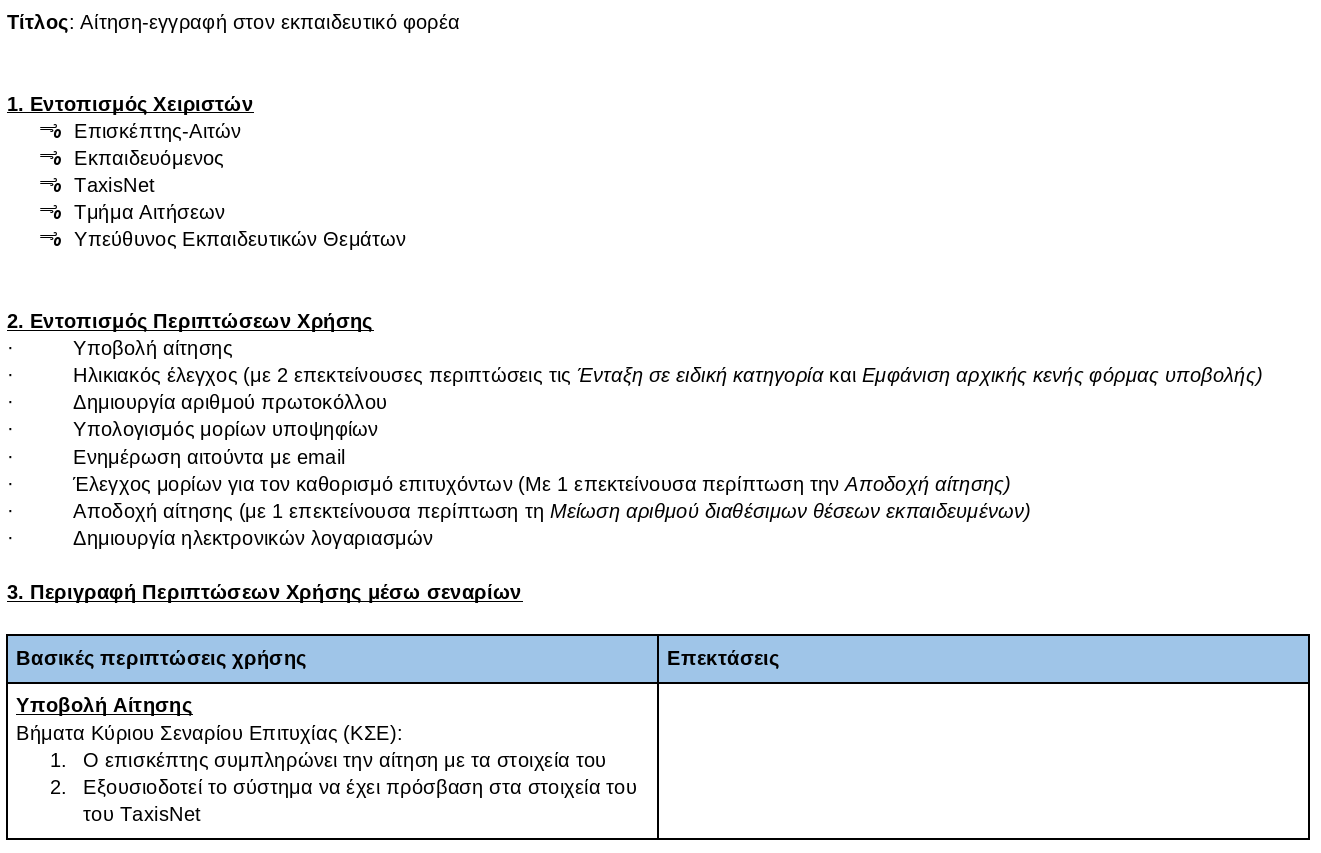
\includegraphics[width=.9\linewidth]{2023-05-31_23-27-36_screenshot.png}
\end{center}
\begin{center}
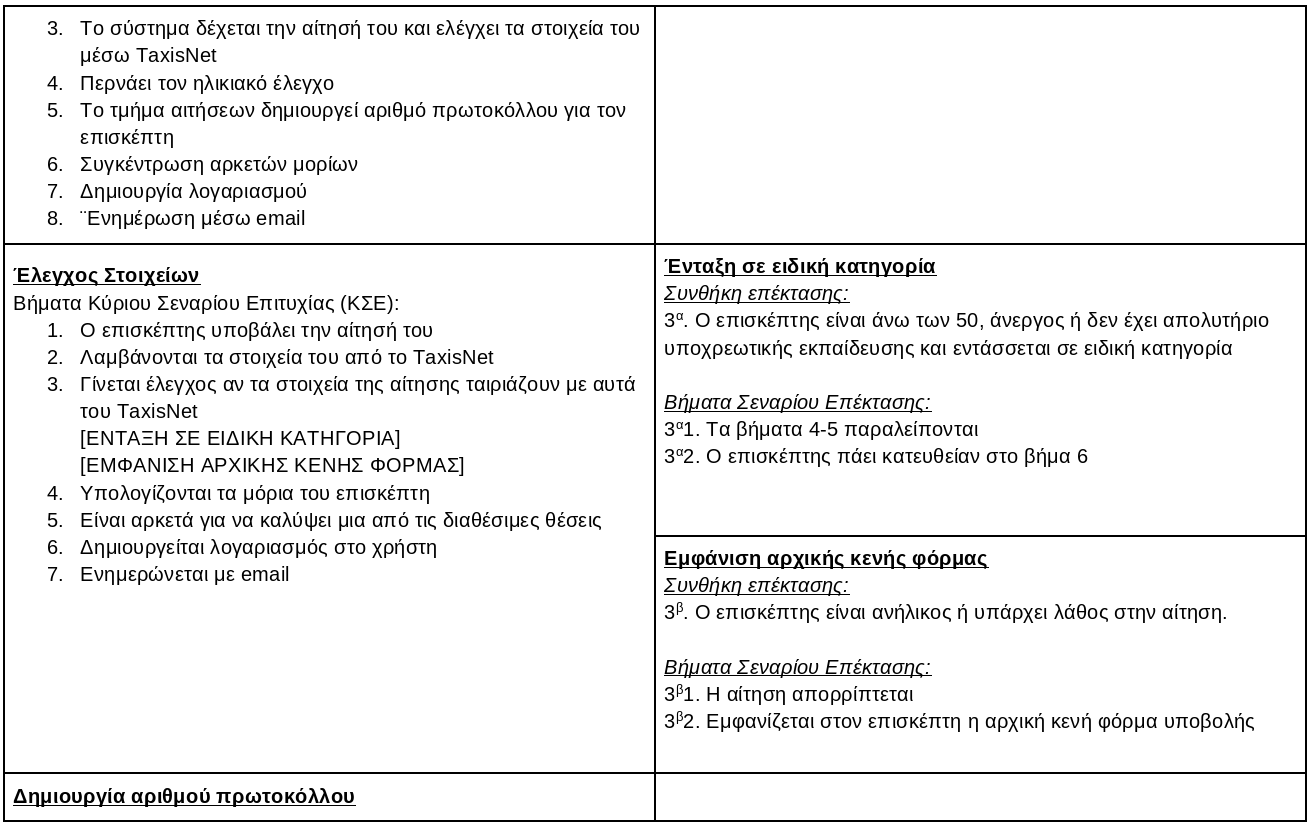
\includegraphics[width=.9\linewidth]{2023-05-31_23-27-45_screenshot.png}
\end{center}
\begin{center}
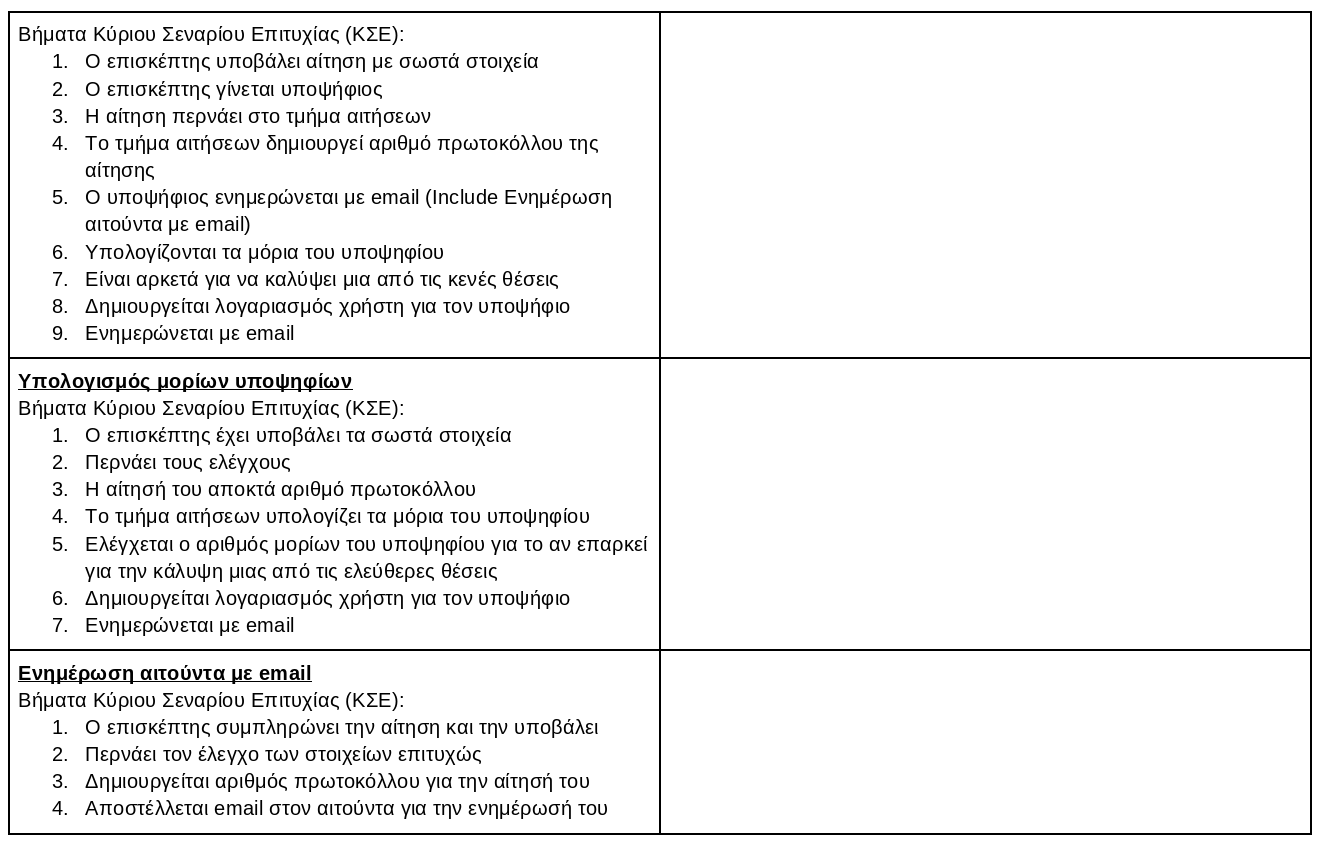
\includegraphics[width=.9\linewidth]{2023-05-31_23-27-53_screenshot.png}
\end{center}
\begin{center}
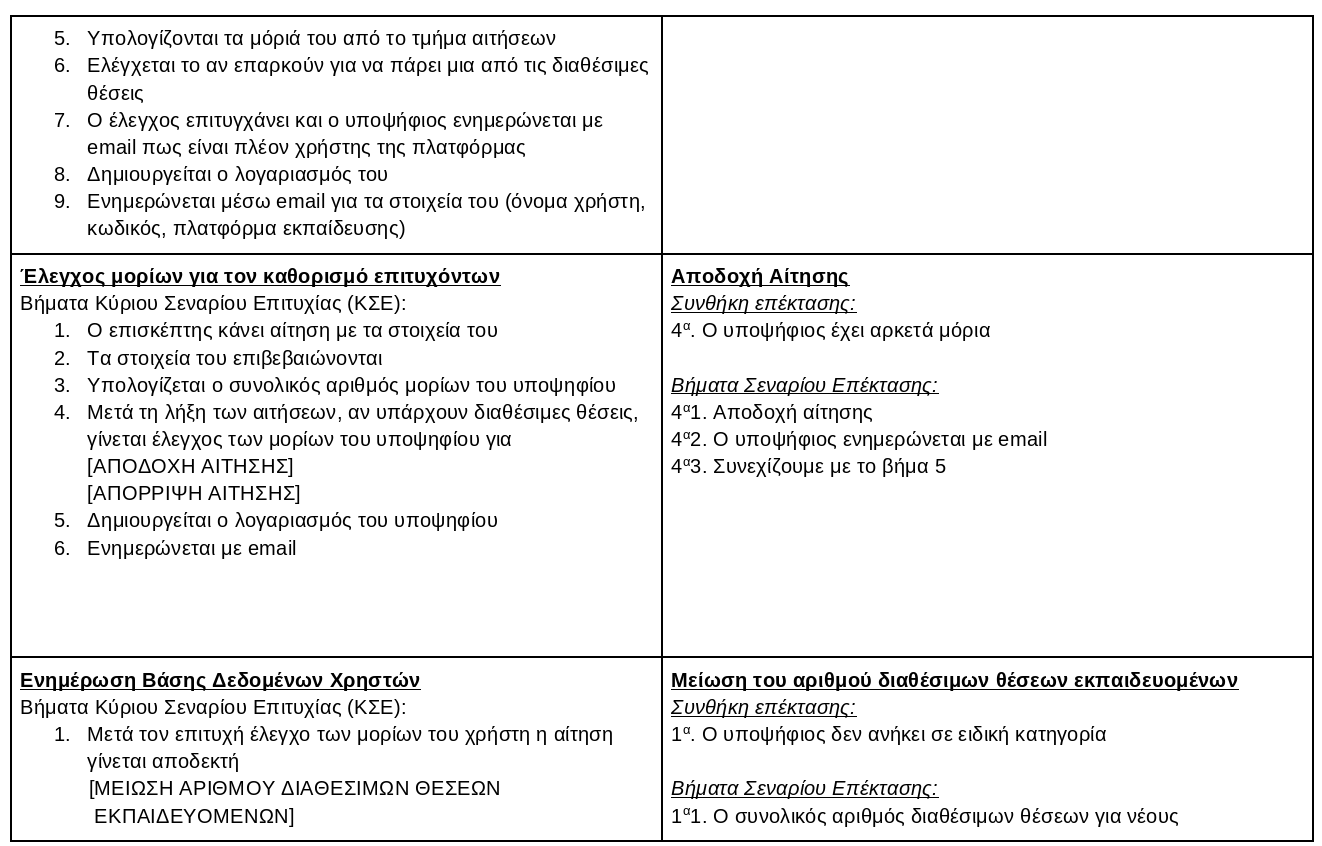
\includegraphics[width=.9\linewidth]{2023-05-31_23-28-00_screenshot.png}
\end{center}
\begin{center}
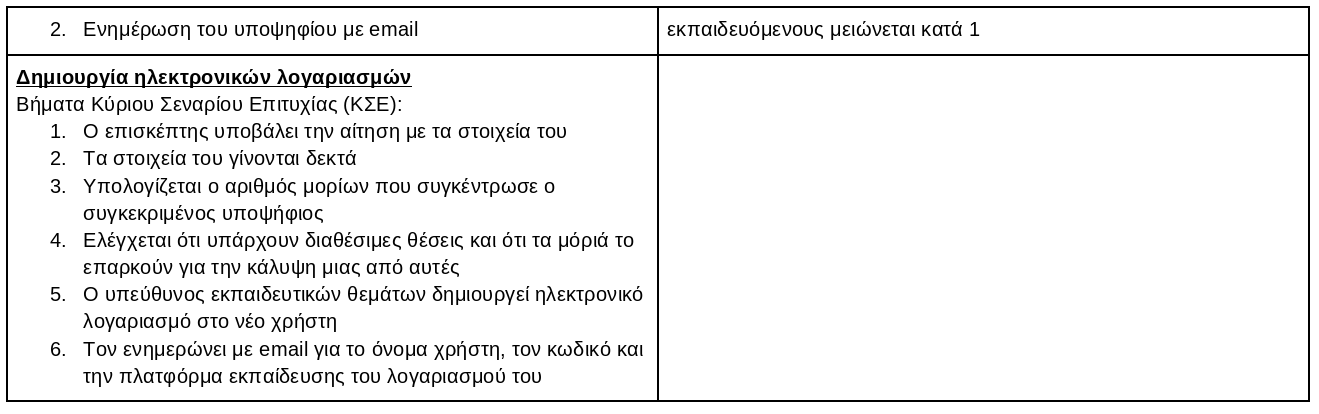
\includegraphics[width=.9\linewidth]{2023-05-31_23-28-07_screenshot.png}
\end{center}

\subsubsection*{Διαγράμματα Περιπτώσεων Χρήσης}
\label{sec:org9c39649}

\begin{itemize}
\item Διαδικασία 1
\label{sec:orgd18cec9}
\begin{center}
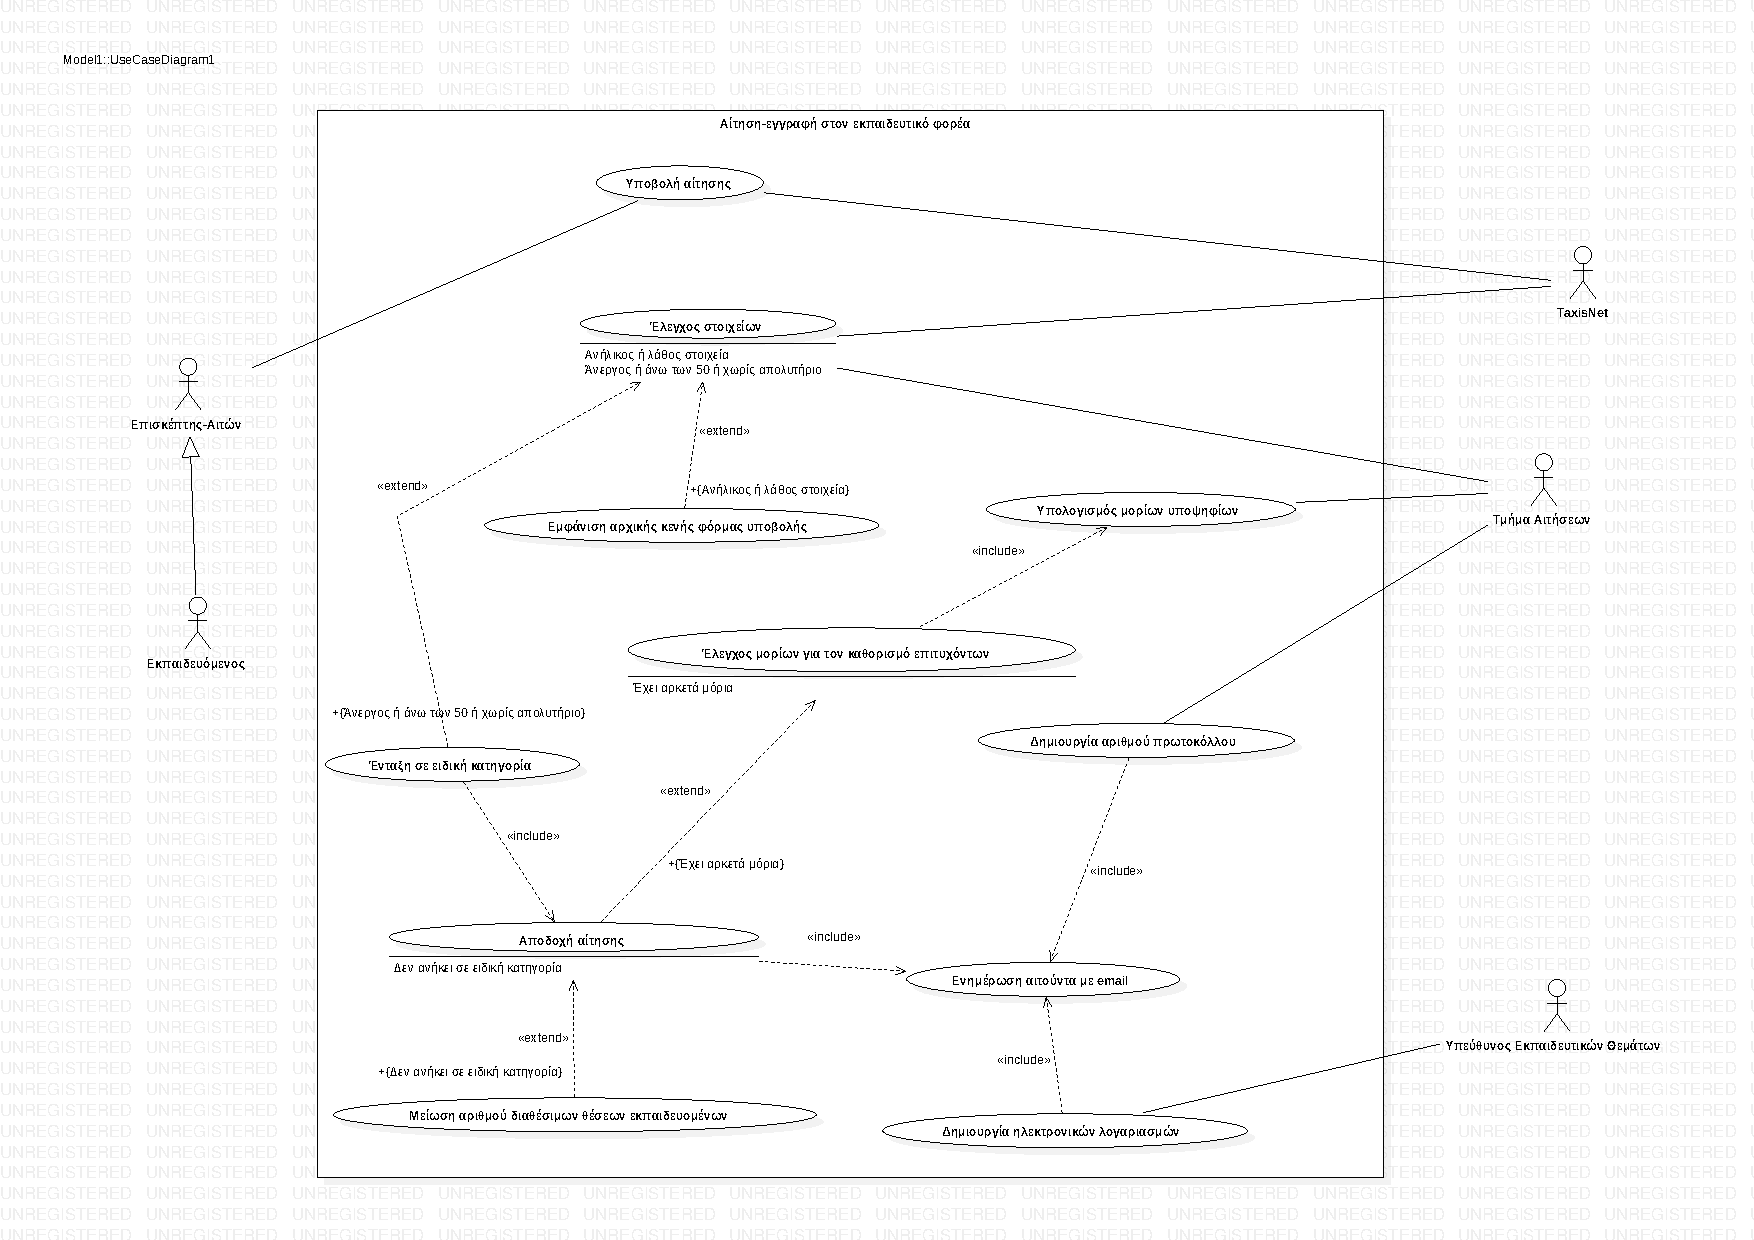
\includegraphics[width=.9\linewidth]{use-case_1.pdf}
\end{center}
\item Διαδικασία 2
\label{sec:org7ca5e81}
\begin{center}
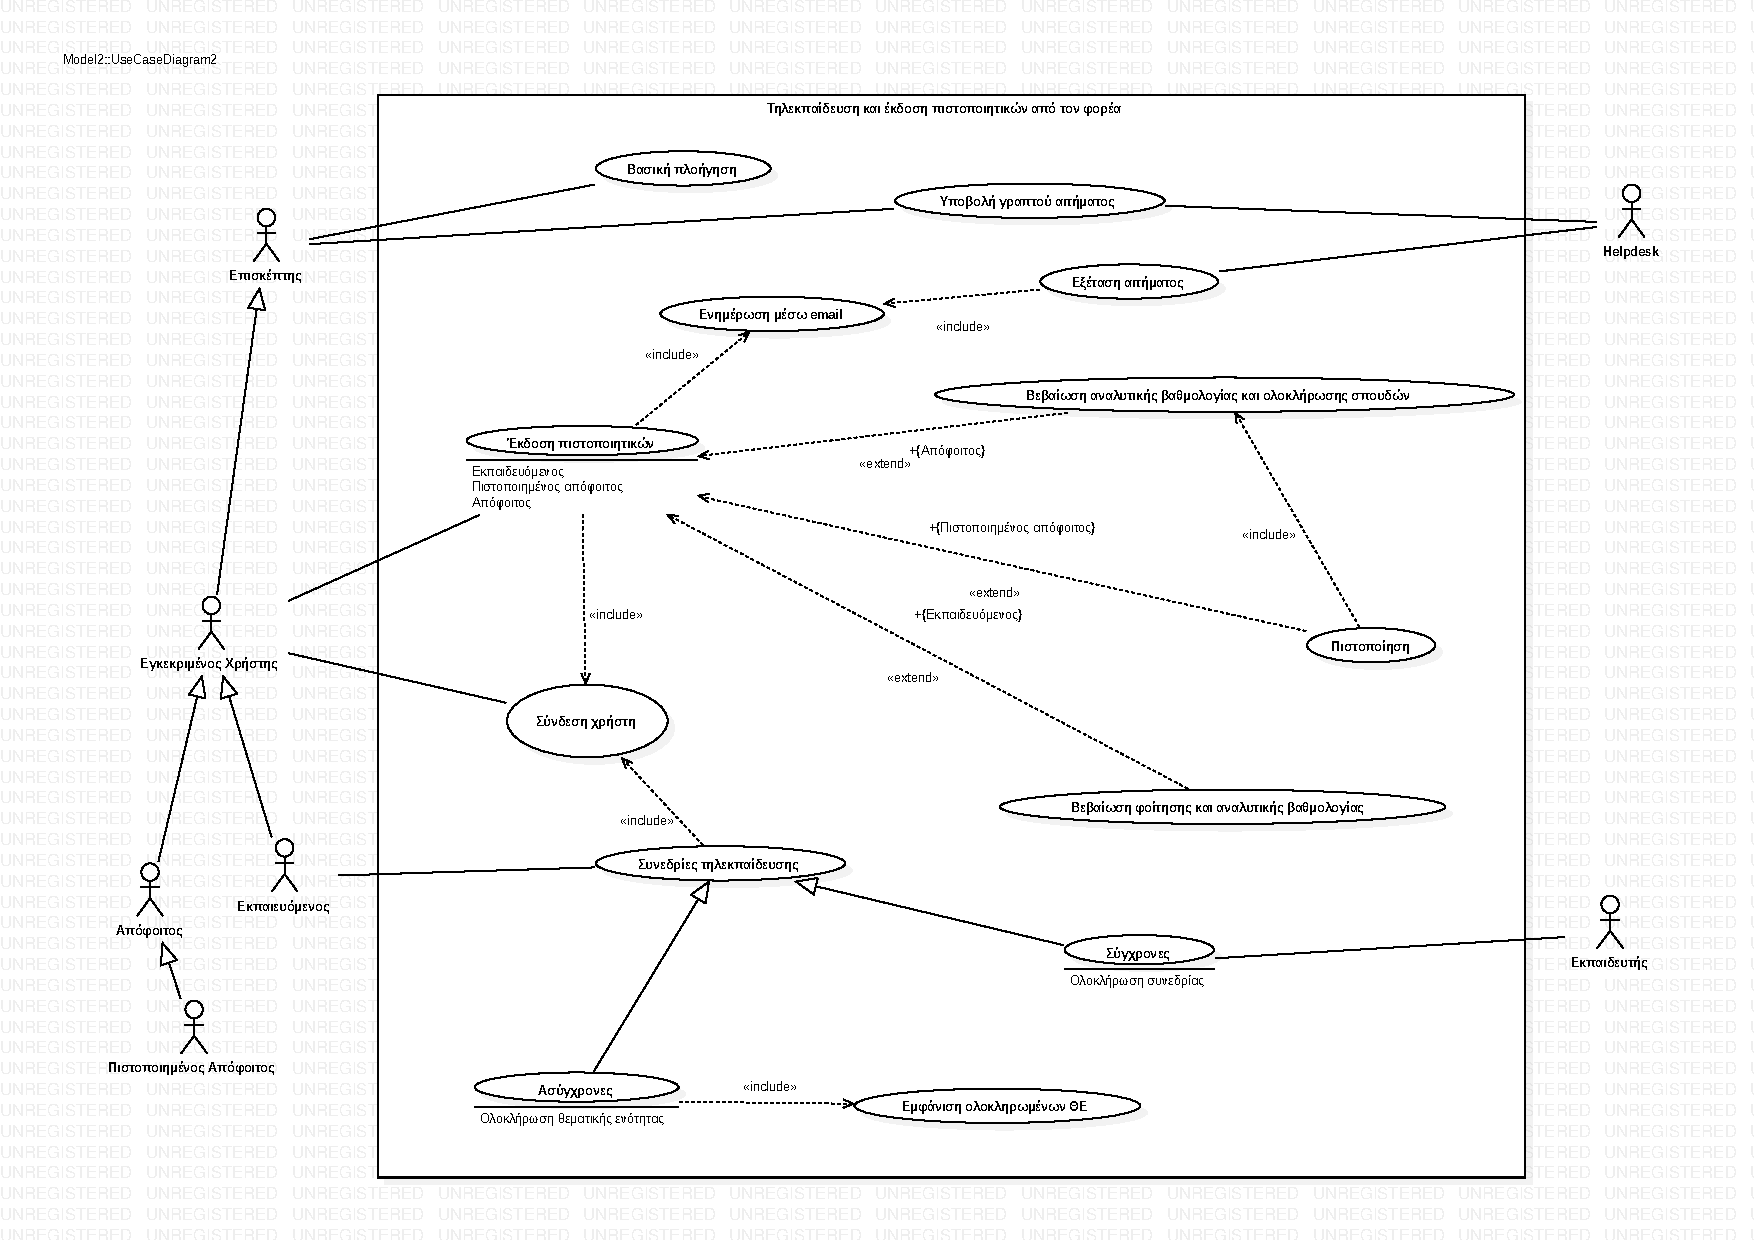
\includegraphics[width=.9\linewidth]{use-case_2.pdf}
\end{center}
\item Διαδικασία 3
\label{sec:org75c7d73}
\begin{center}
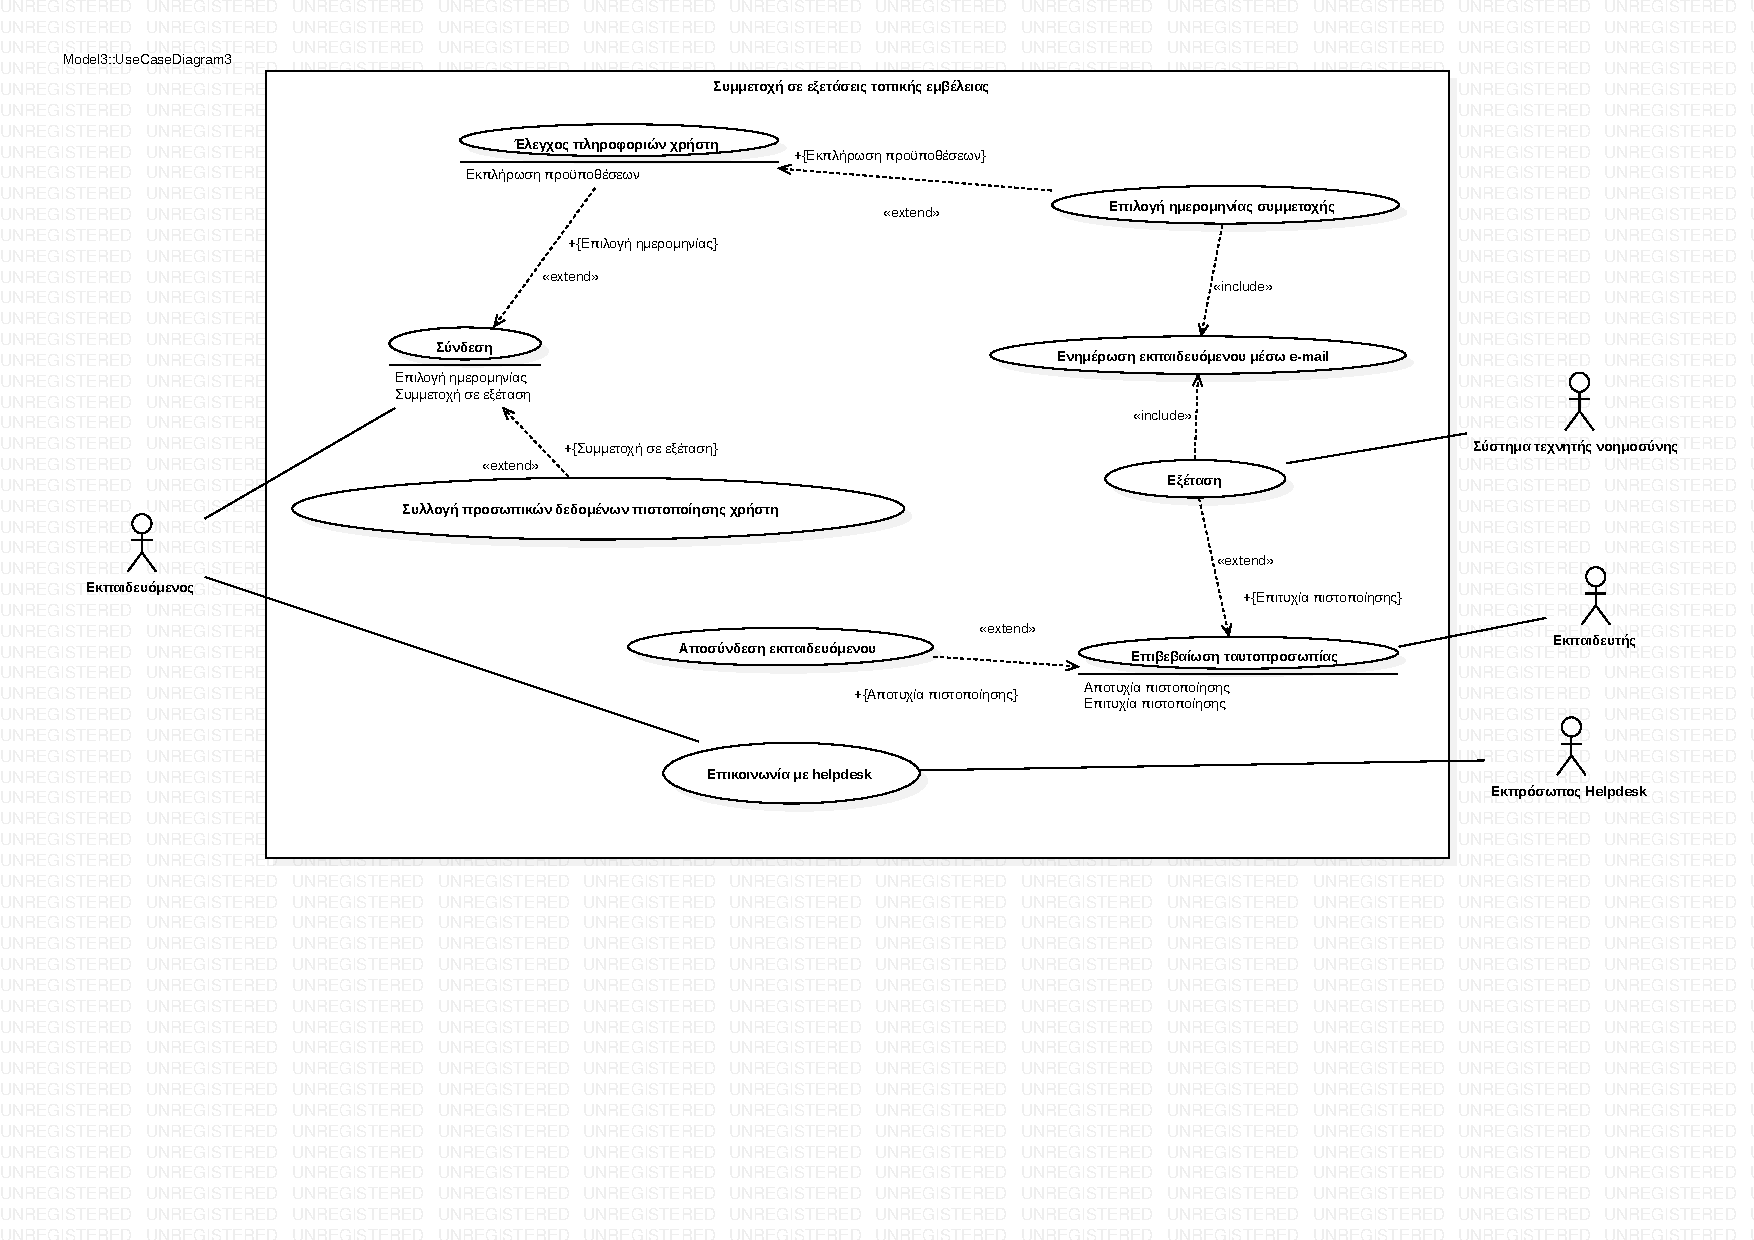
\includegraphics[width=.9\linewidth]{use-case_3.pdf}
\end{center}
\item Διαδικασία 4
\label{sec:orgf548b38}
\begin{center}
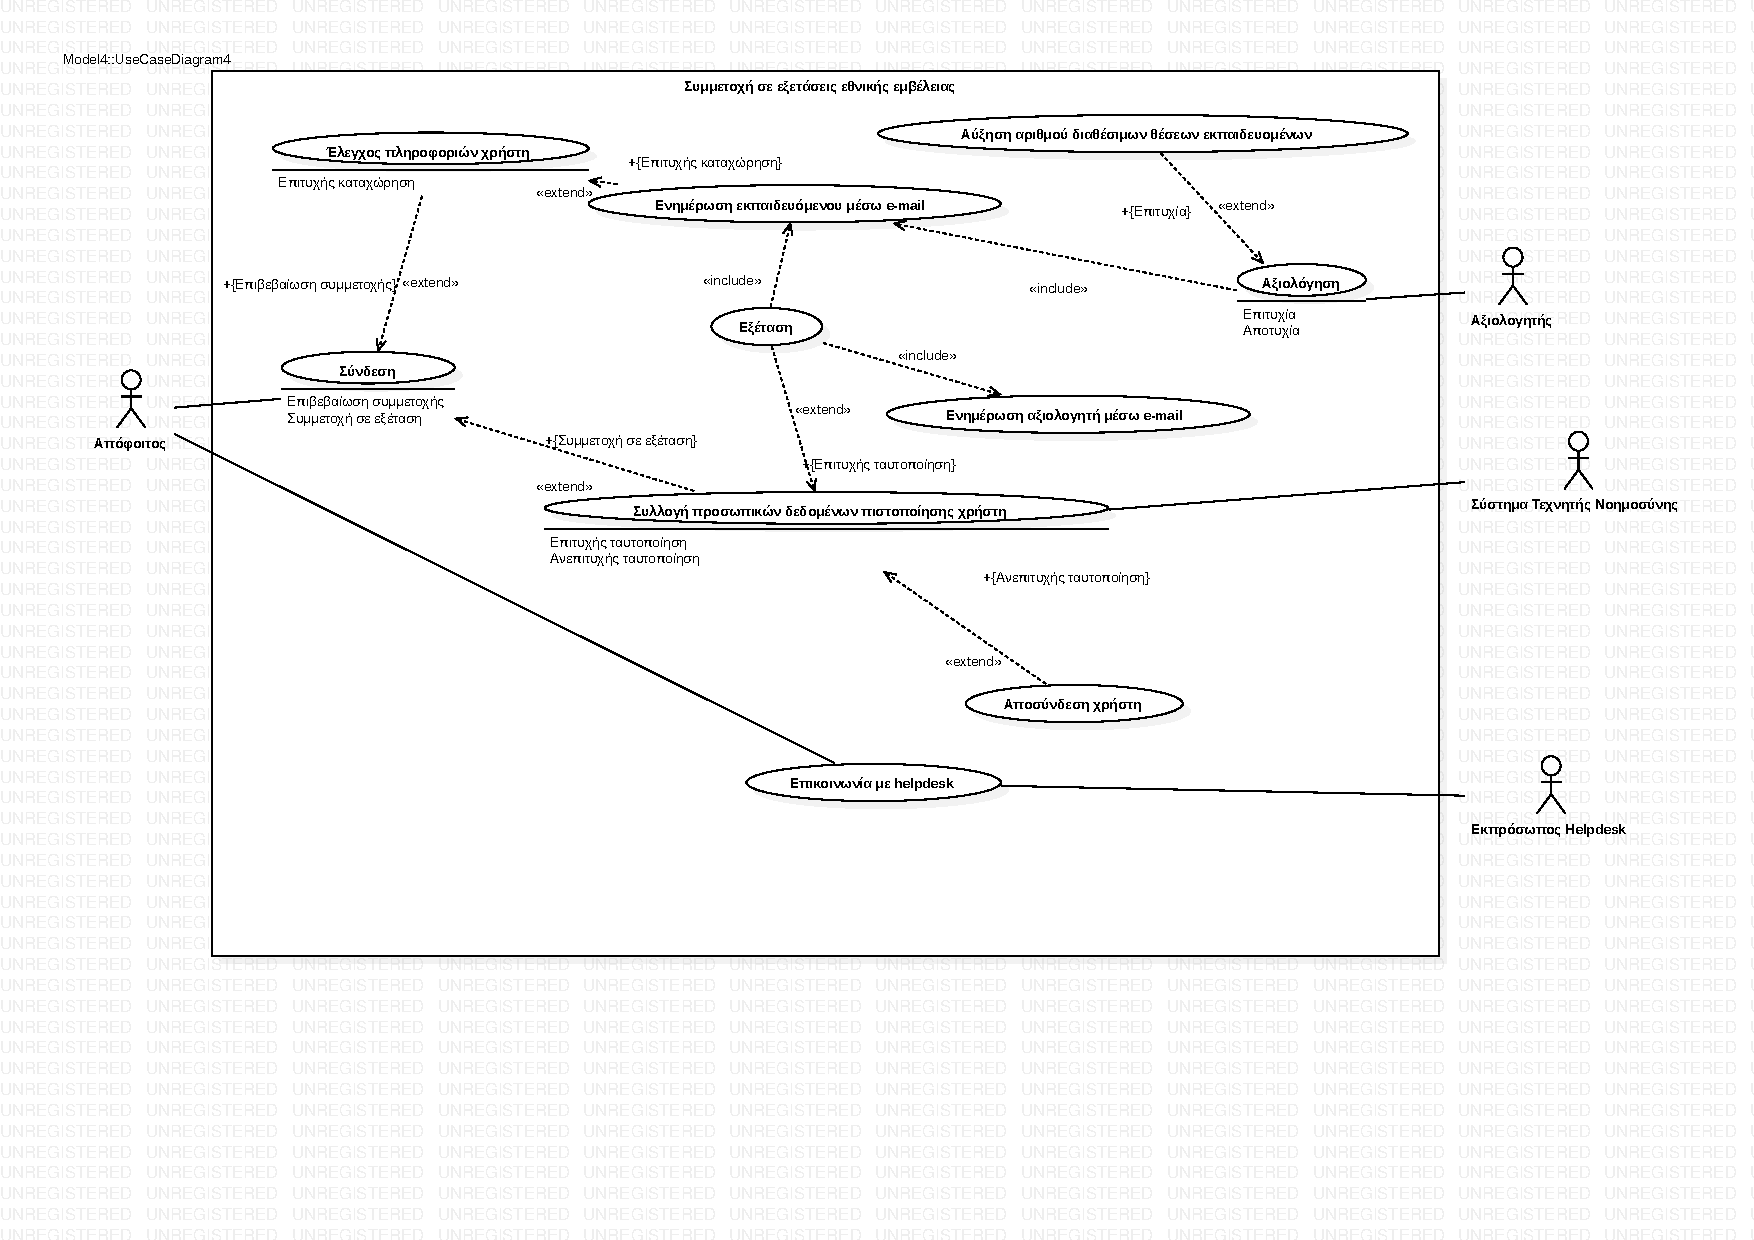
\includegraphics[width=.9\linewidth]{use-case_4.pdf}
\end{center}
\end{itemize}

\subsection{Ερώτημα 2}
\label{sec:org9dddf03}

\subsubsection*{Διαγράμματα Κλάσεων}
\label{sec:orgc4066d0}

\begin{itemize}
\item Διαδικασία 1
\label{sec:orgb01ed71}
\begin{center}
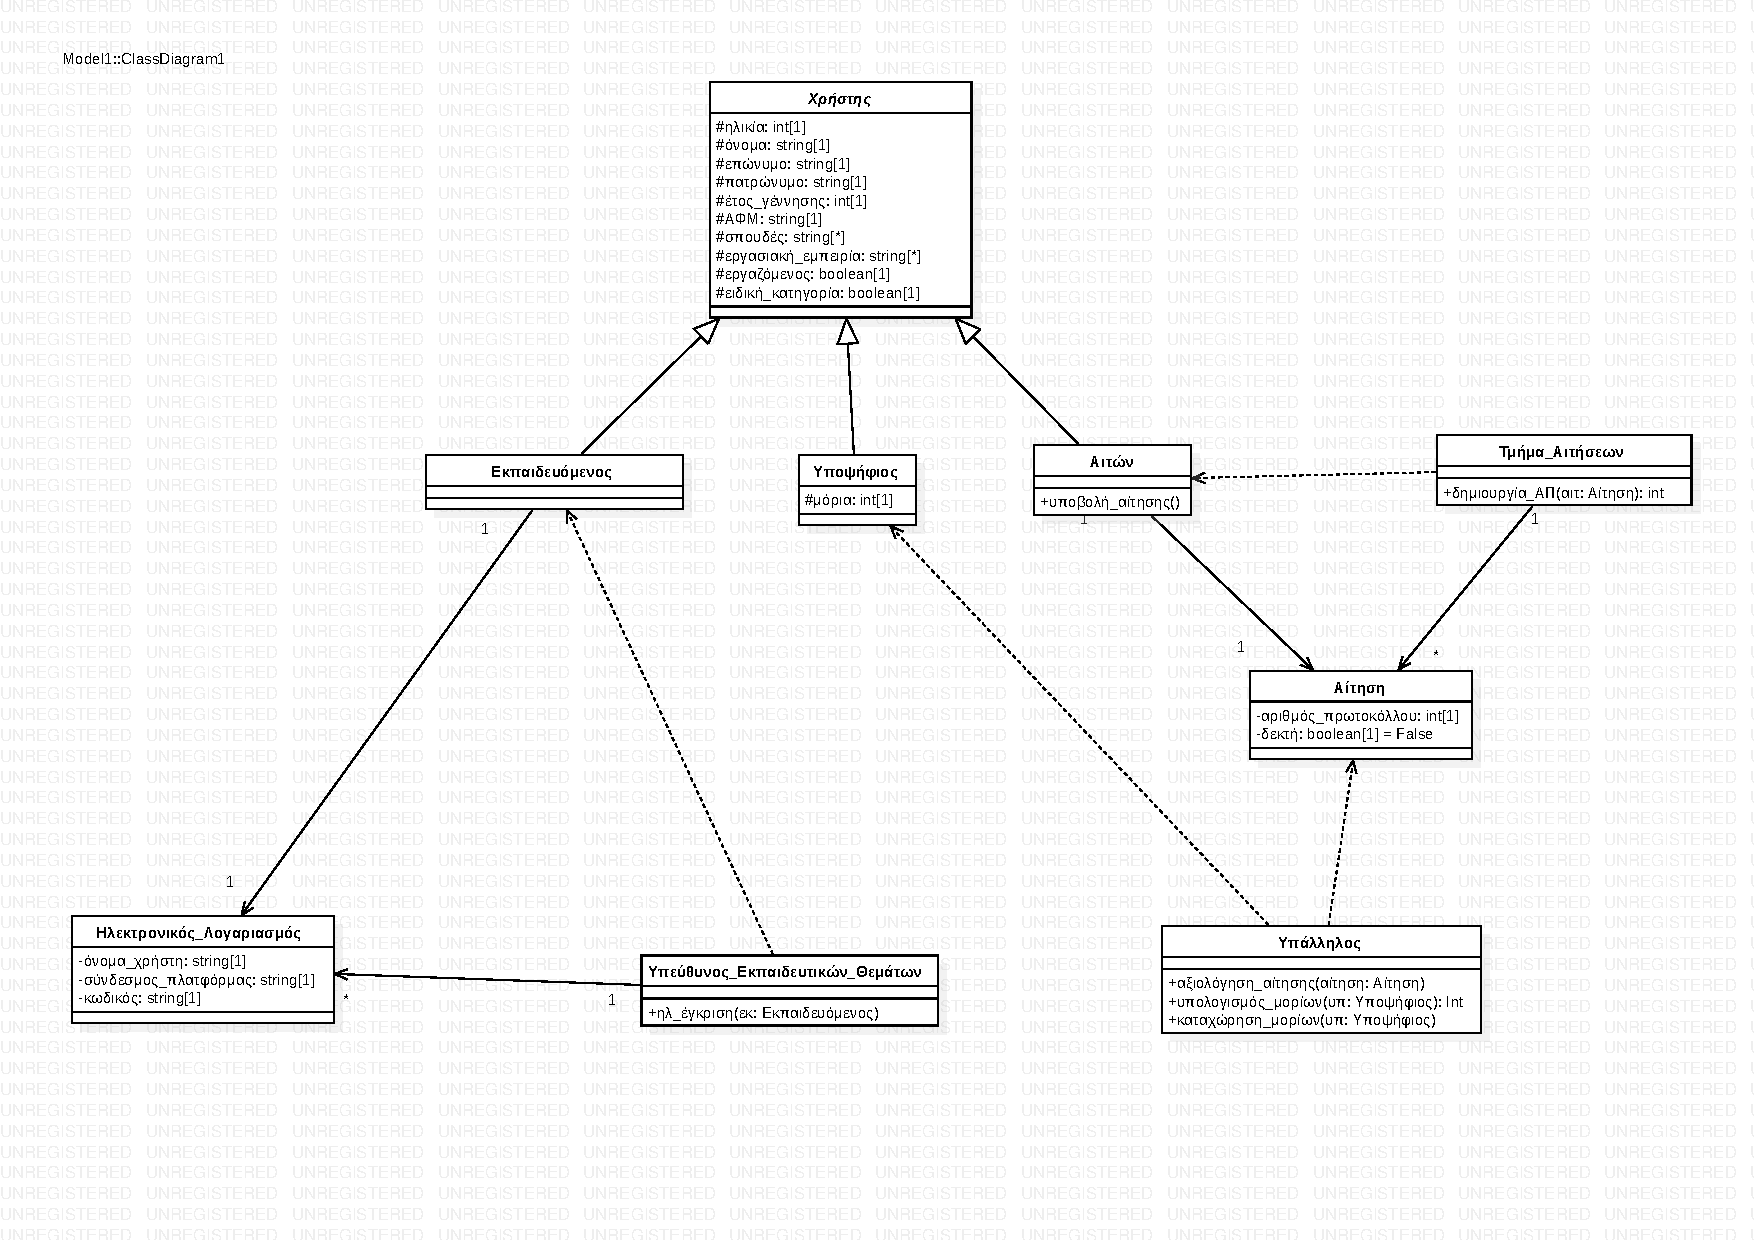
\includegraphics[width=.9\linewidth]{class_1.pdf}
\end{center}
\item Διαδικασία 2
\label{sec:orgb926db2}
\begin{center}
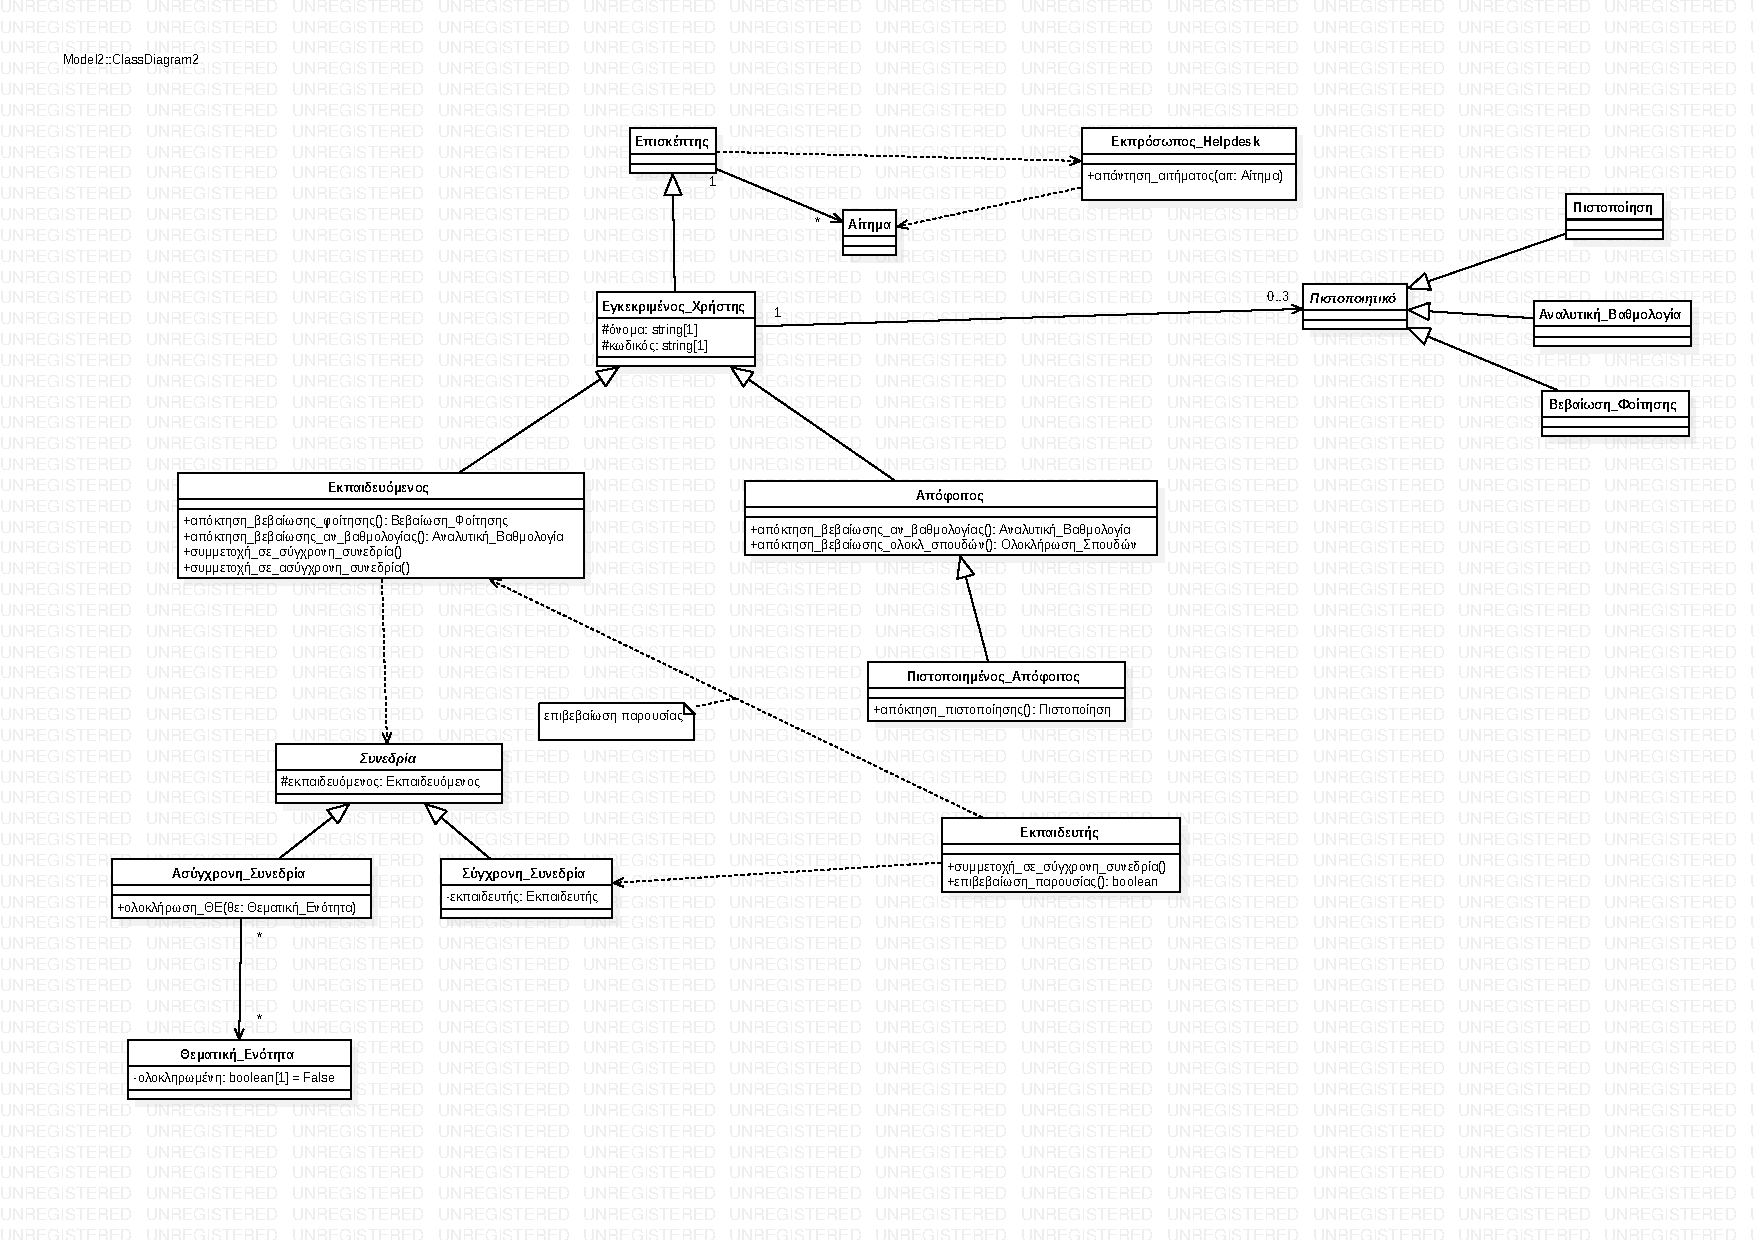
\includegraphics[width=.9\linewidth]{class_2.pdf}
\end{center}
\item Διαδικασία 3
\label{sec:org6dc5efa}
\begin{center}
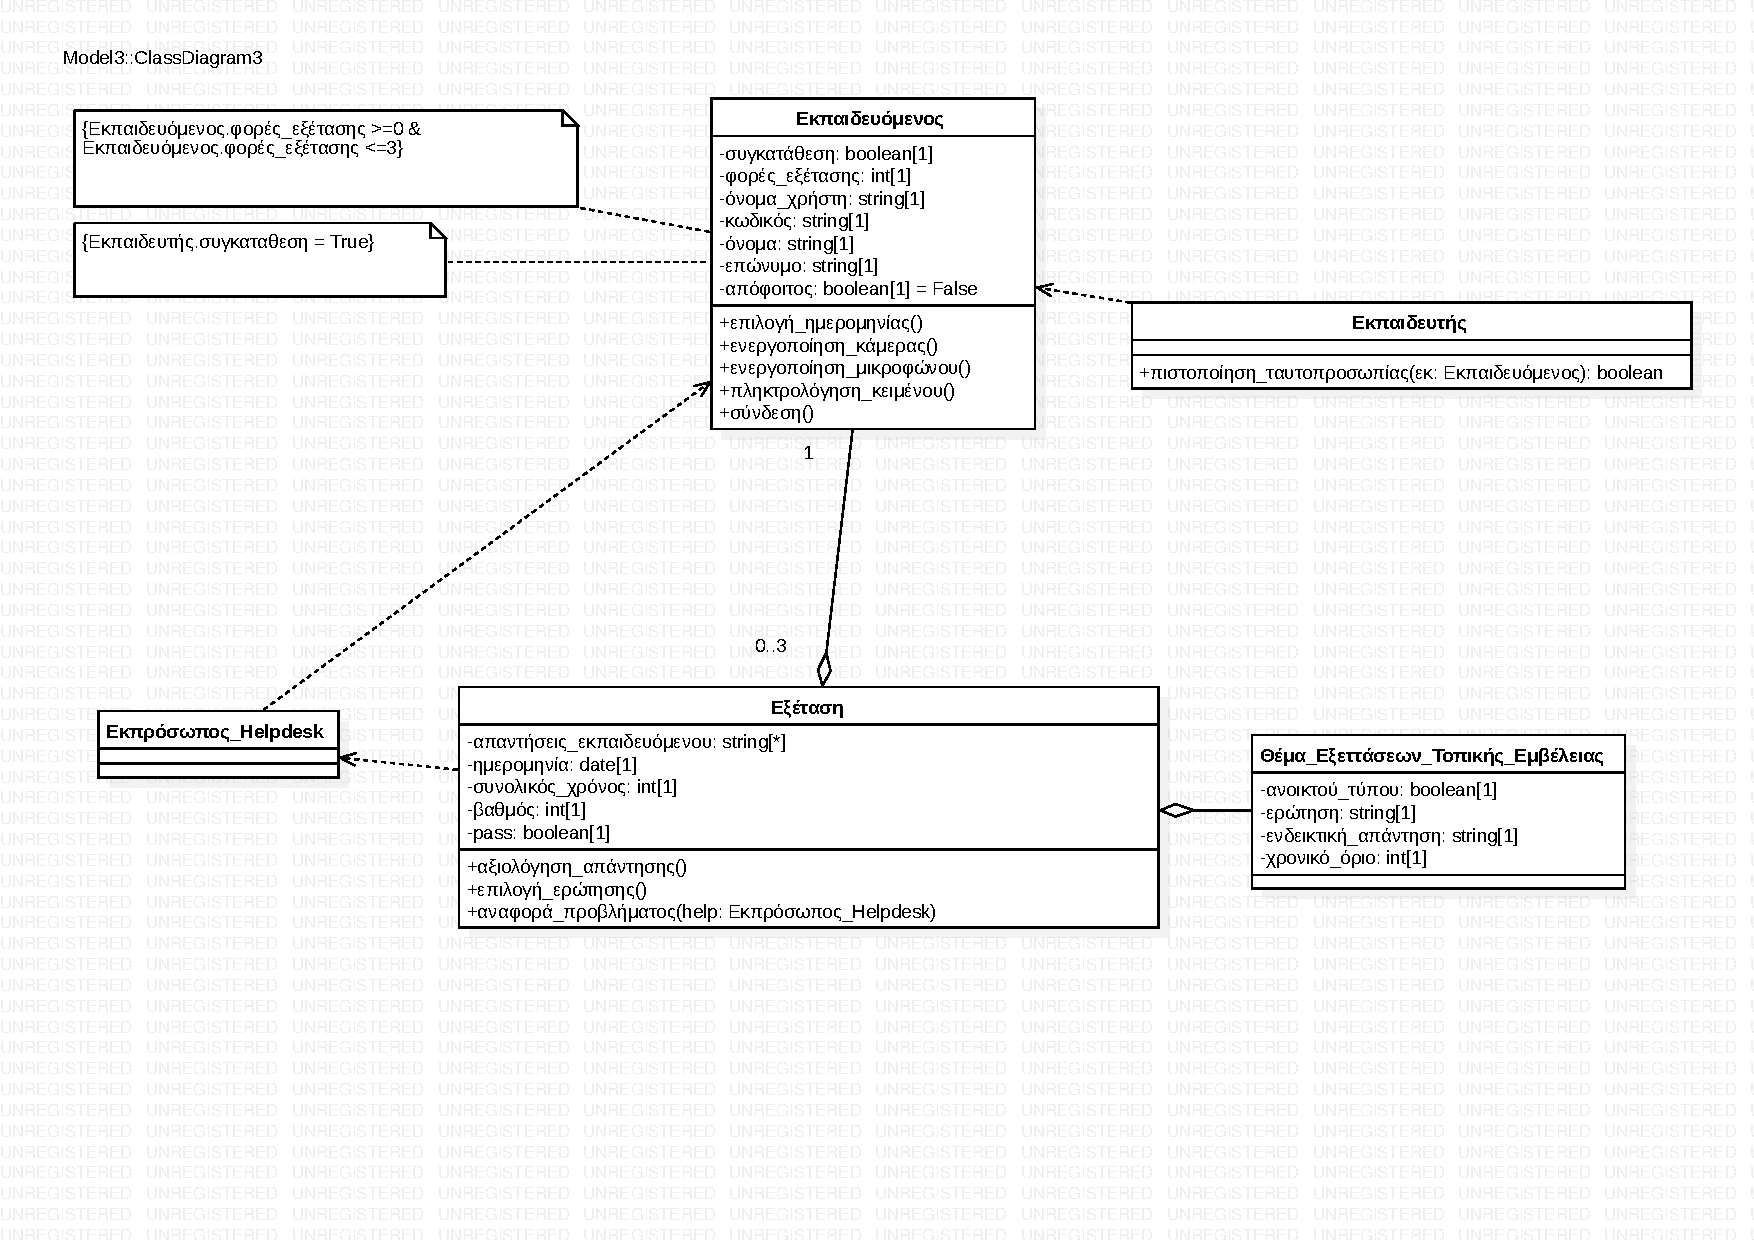
\includegraphics[width=.9\linewidth]{class_3.pdf}
\end{center}
\item Διαδικασία 4
\label{sec:orgfa1d02e}
\begin{center}
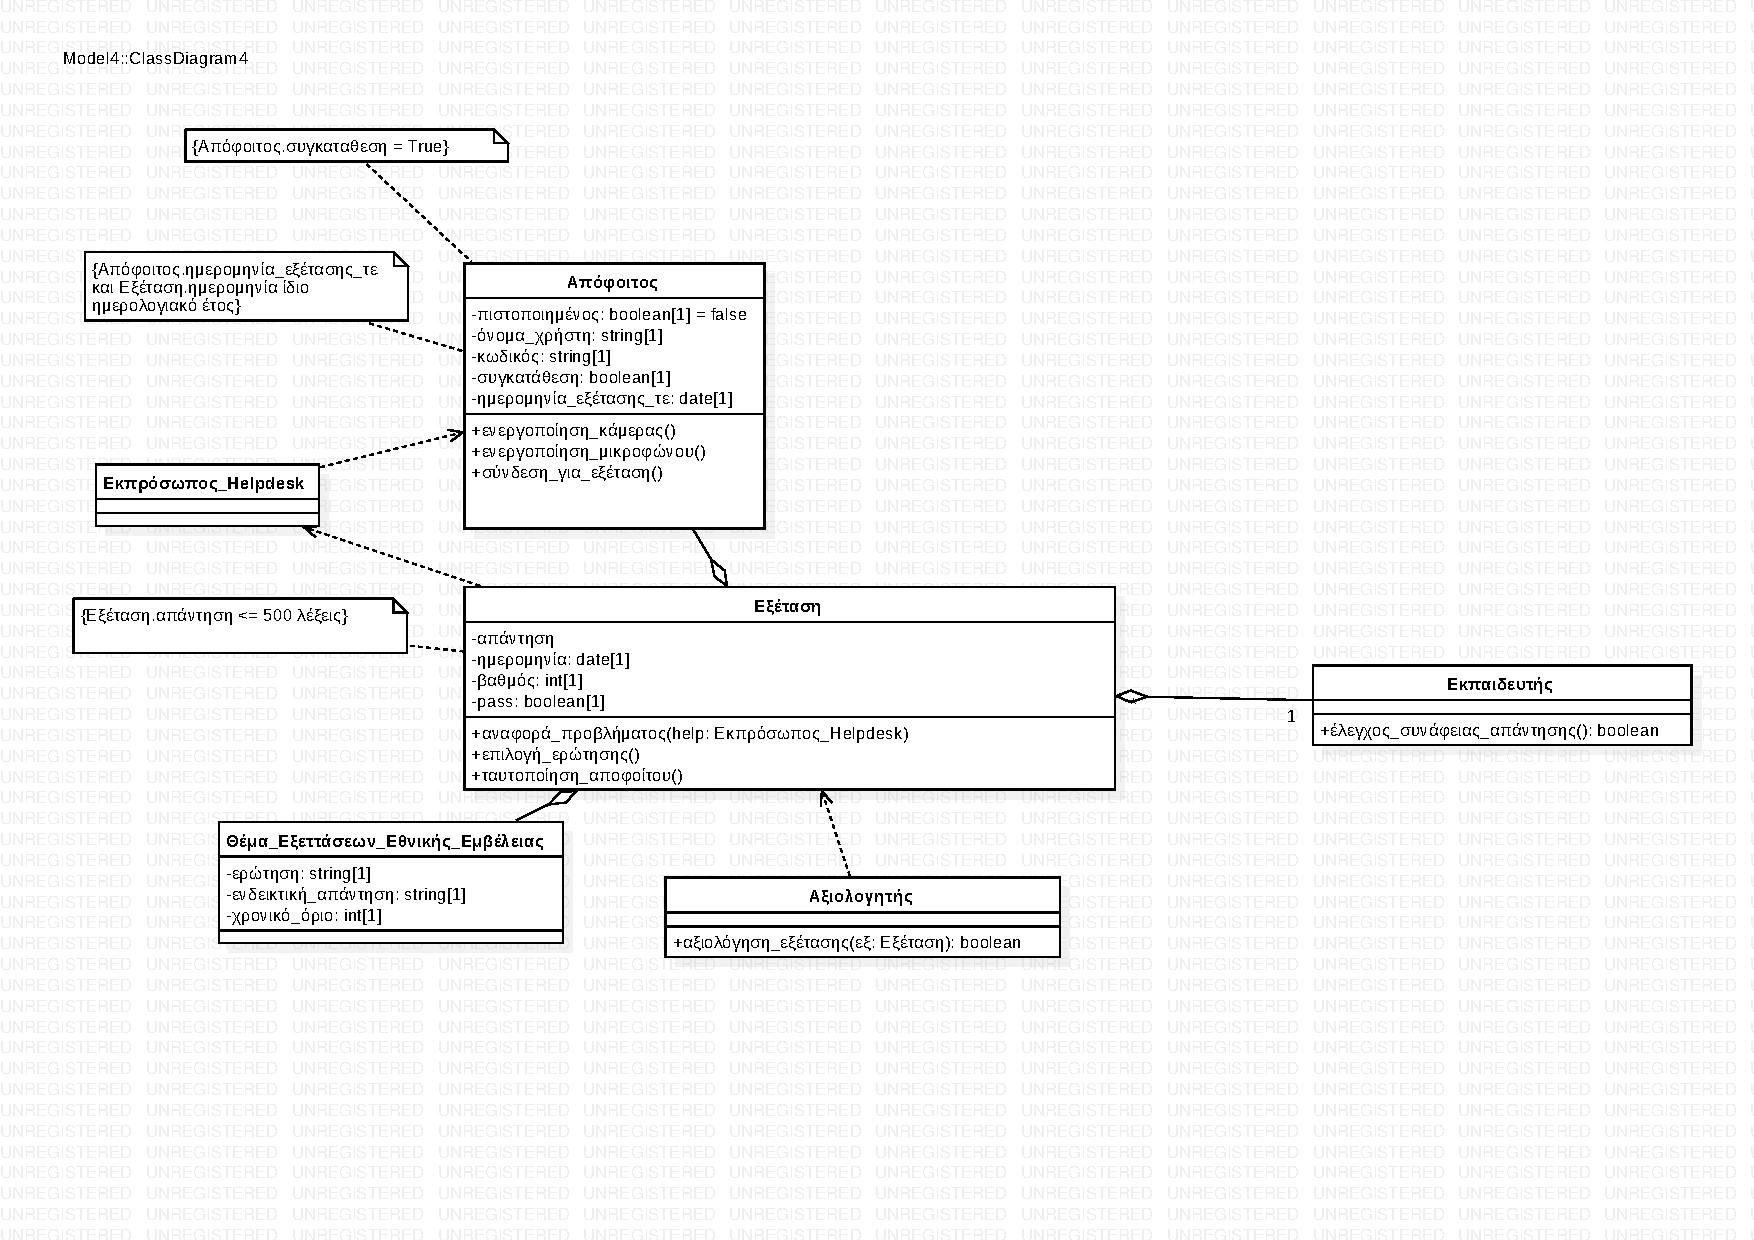
\includegraphics[width=.9\linewidth]{class_4.pdf}
\end{center}
\end{itemize}

\subsection{Ερώτημα 3}
\label{sec:org61d701c}

\begin{center}
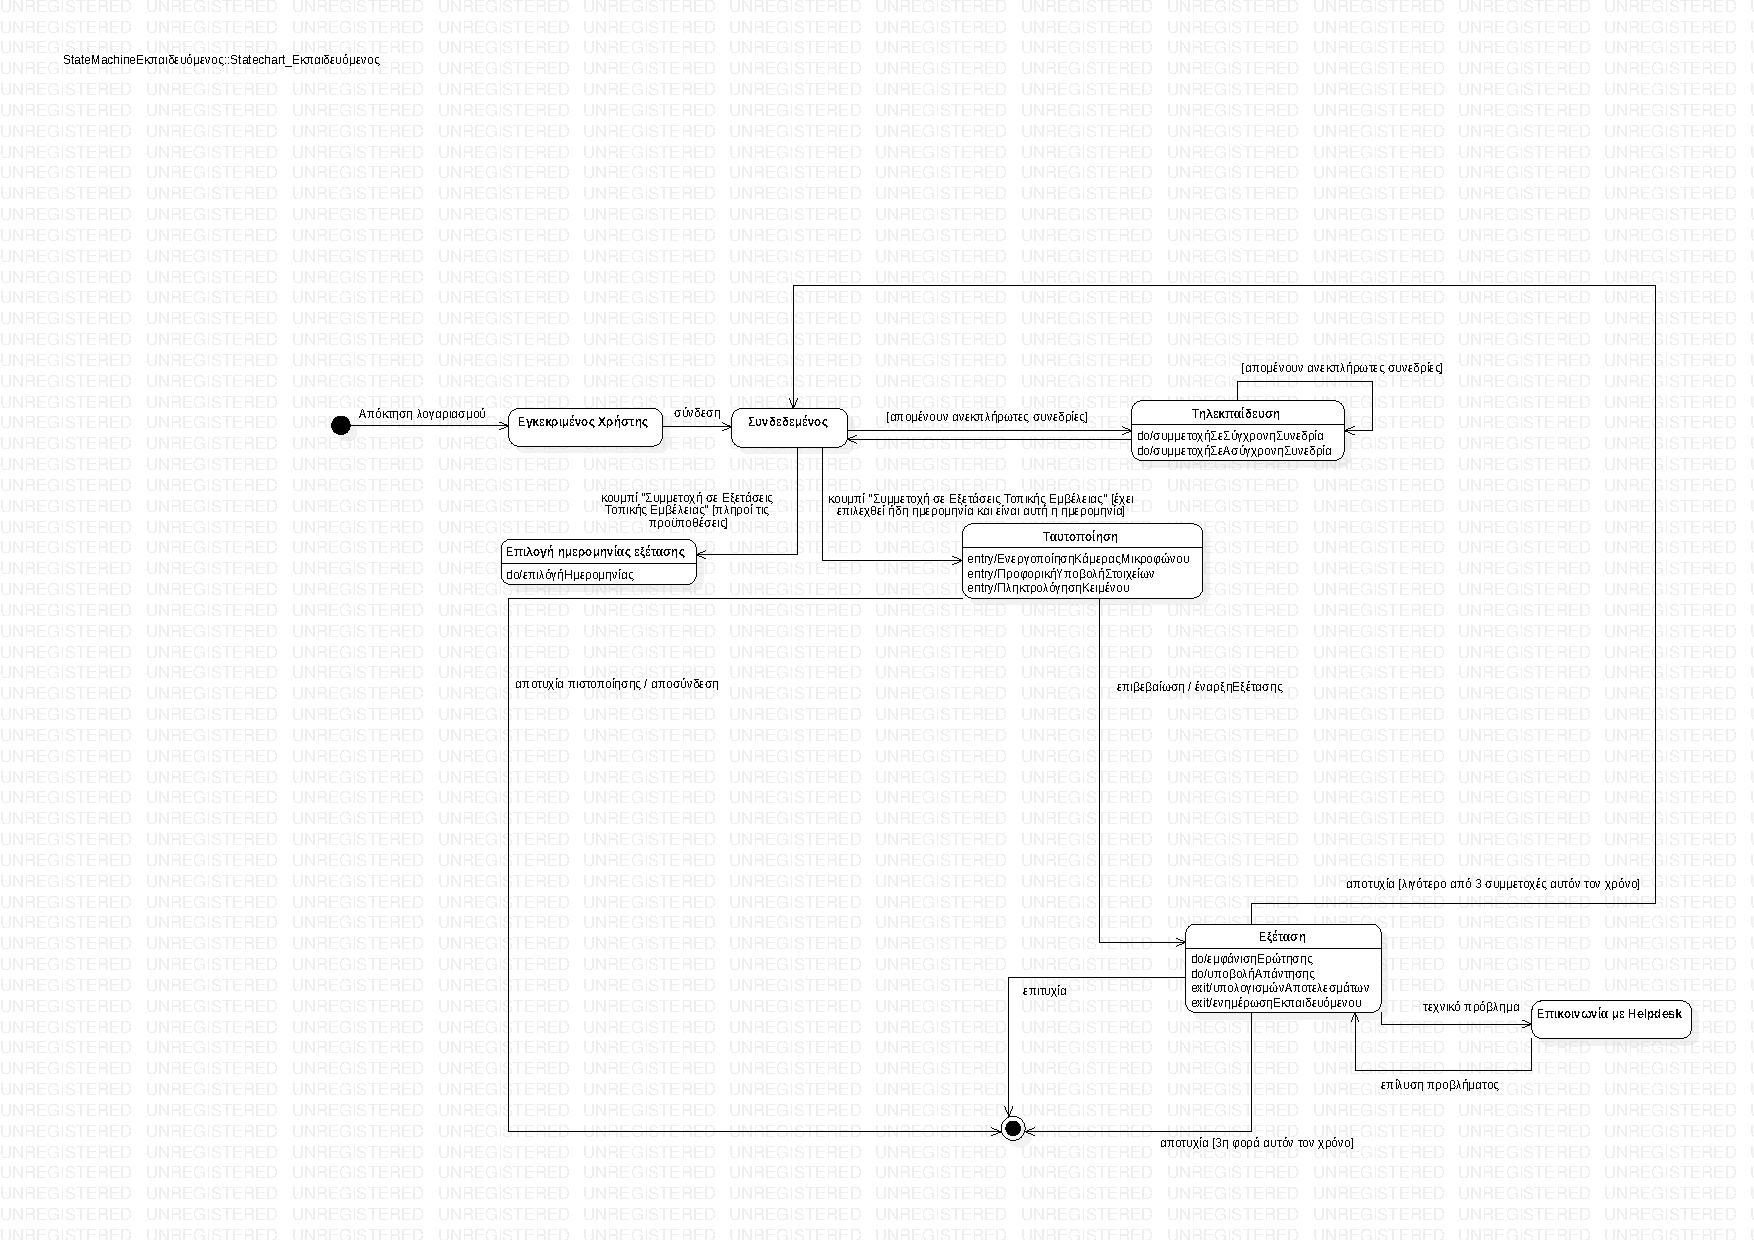
\includegraphics[width=.9\linewidth]{state.pdf}
\end{center}

\subsection{Ερώτημα 4}
\label{sec:org89c2962}

\begin{itemize}
\item Διαδικασία 1
\label{sec:org95b3fb4}
\begin{center}
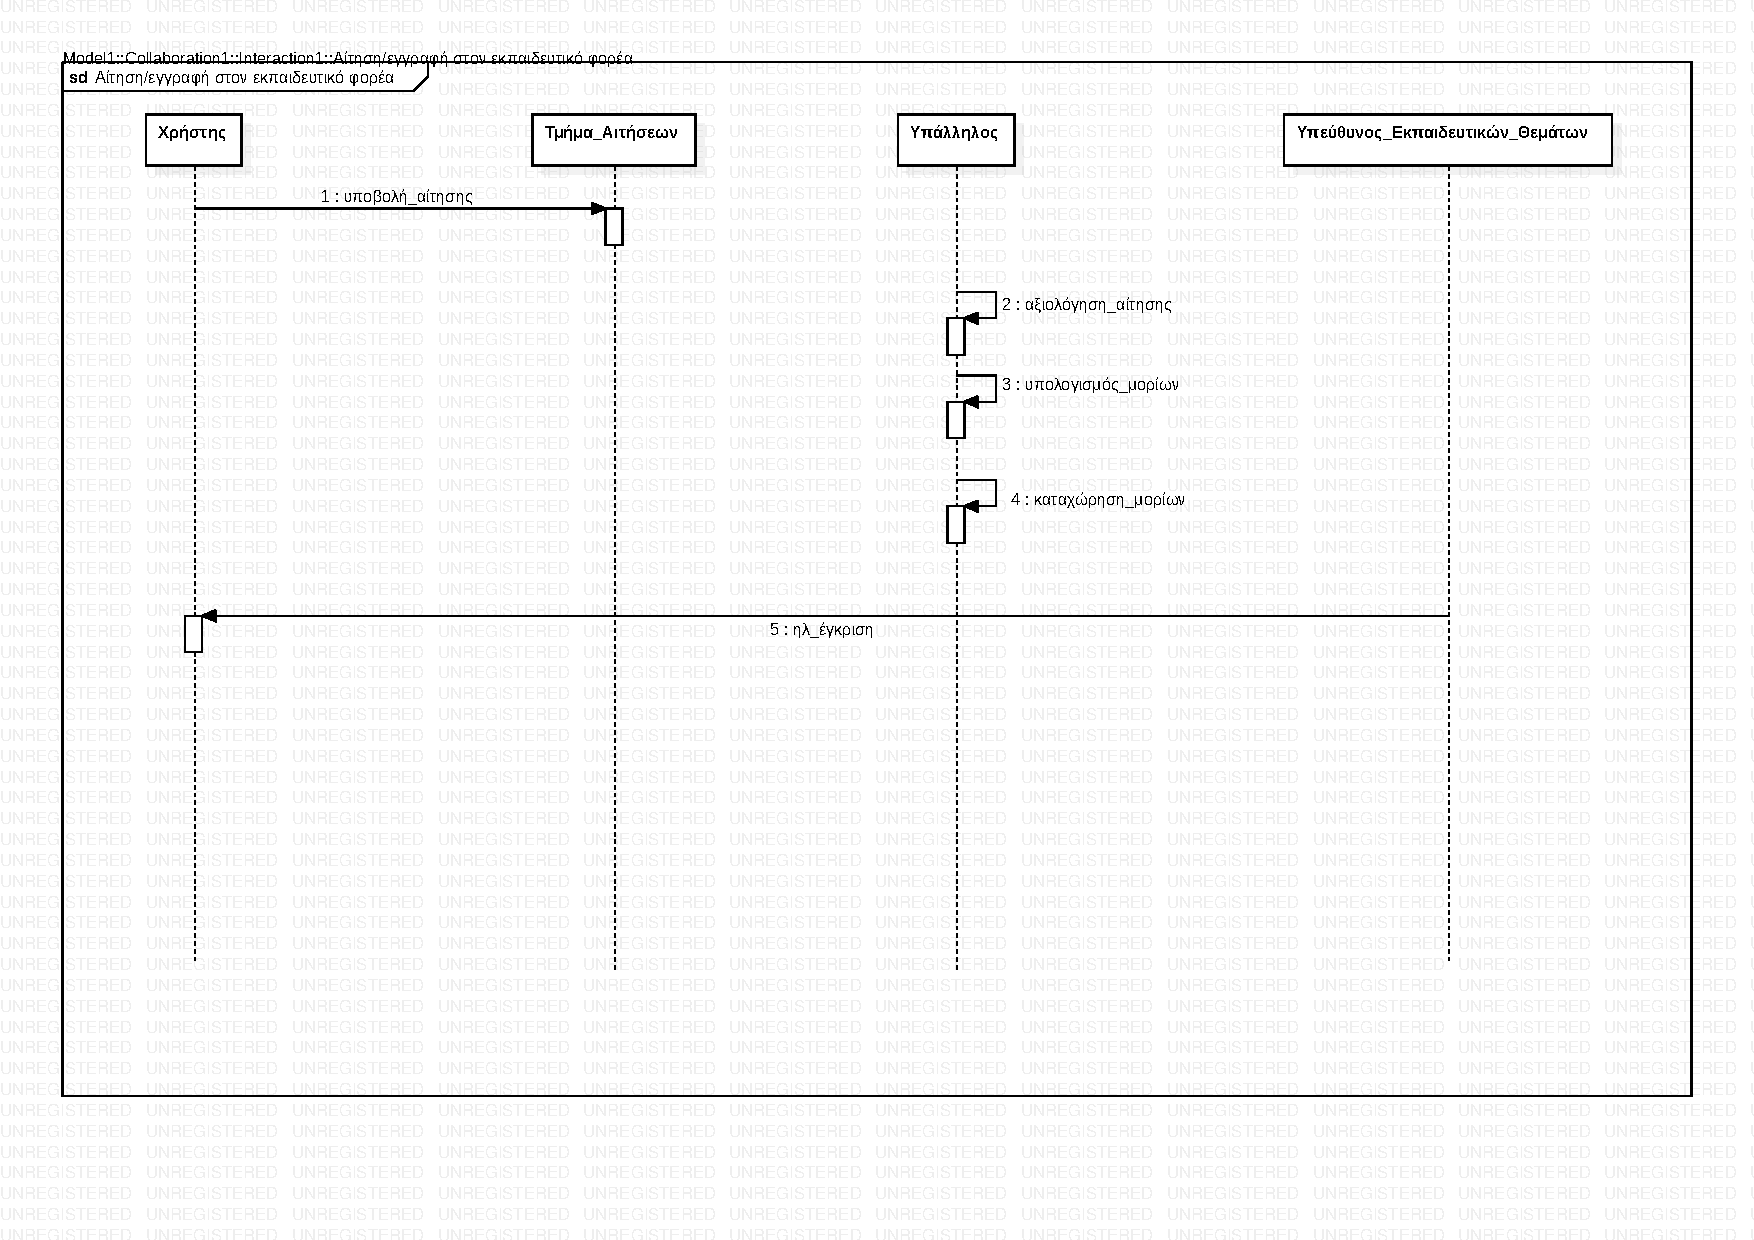
\includegraphics[width=.9\linewidth]{seq_1.pdf}
\end{center}
\item Διαδικασία 3
\label{sec:org3c300ea}
\begin{center}
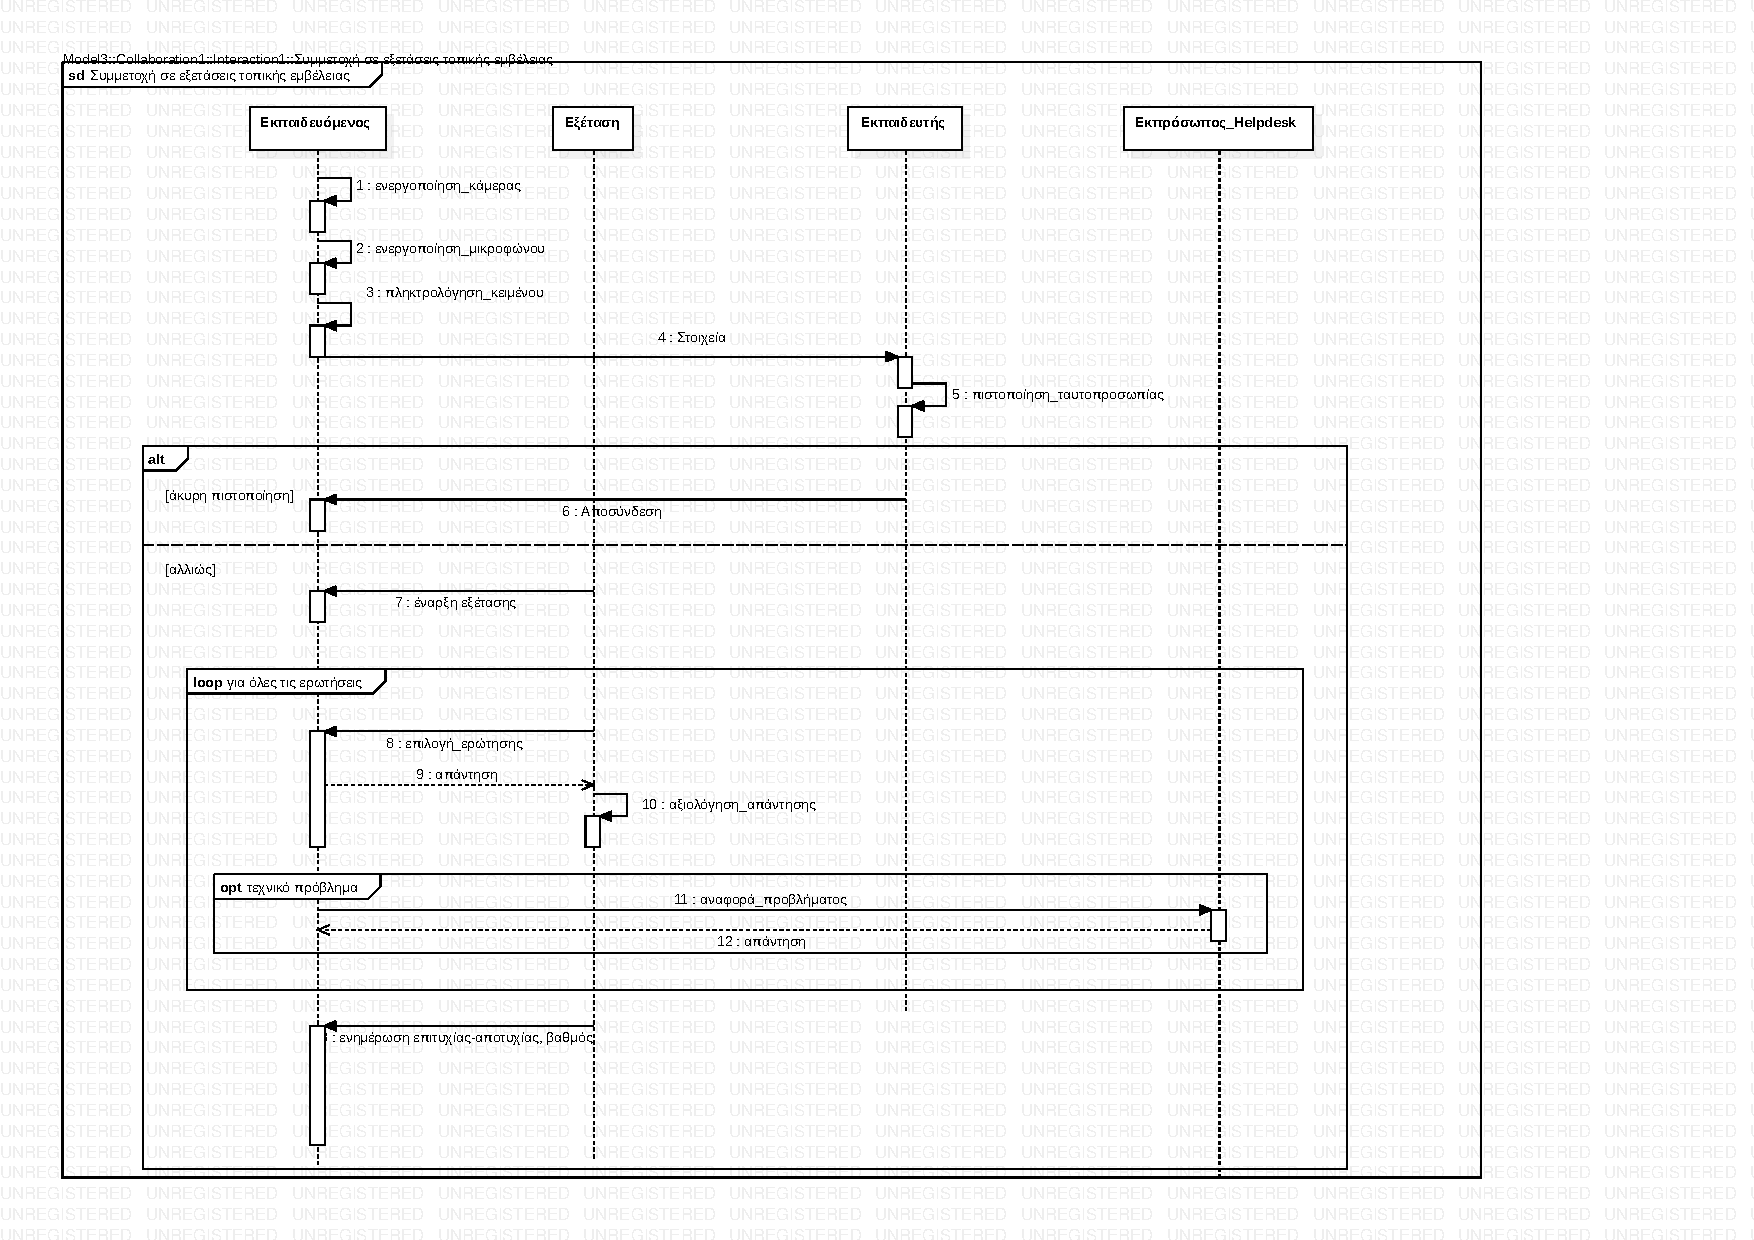
\includegraphics[width=.9\linewidth]{seq_3.pdf}
\end{center}
\item Διαδικασία 4
\label{sec:org0f8cf4e}
\begin{center}
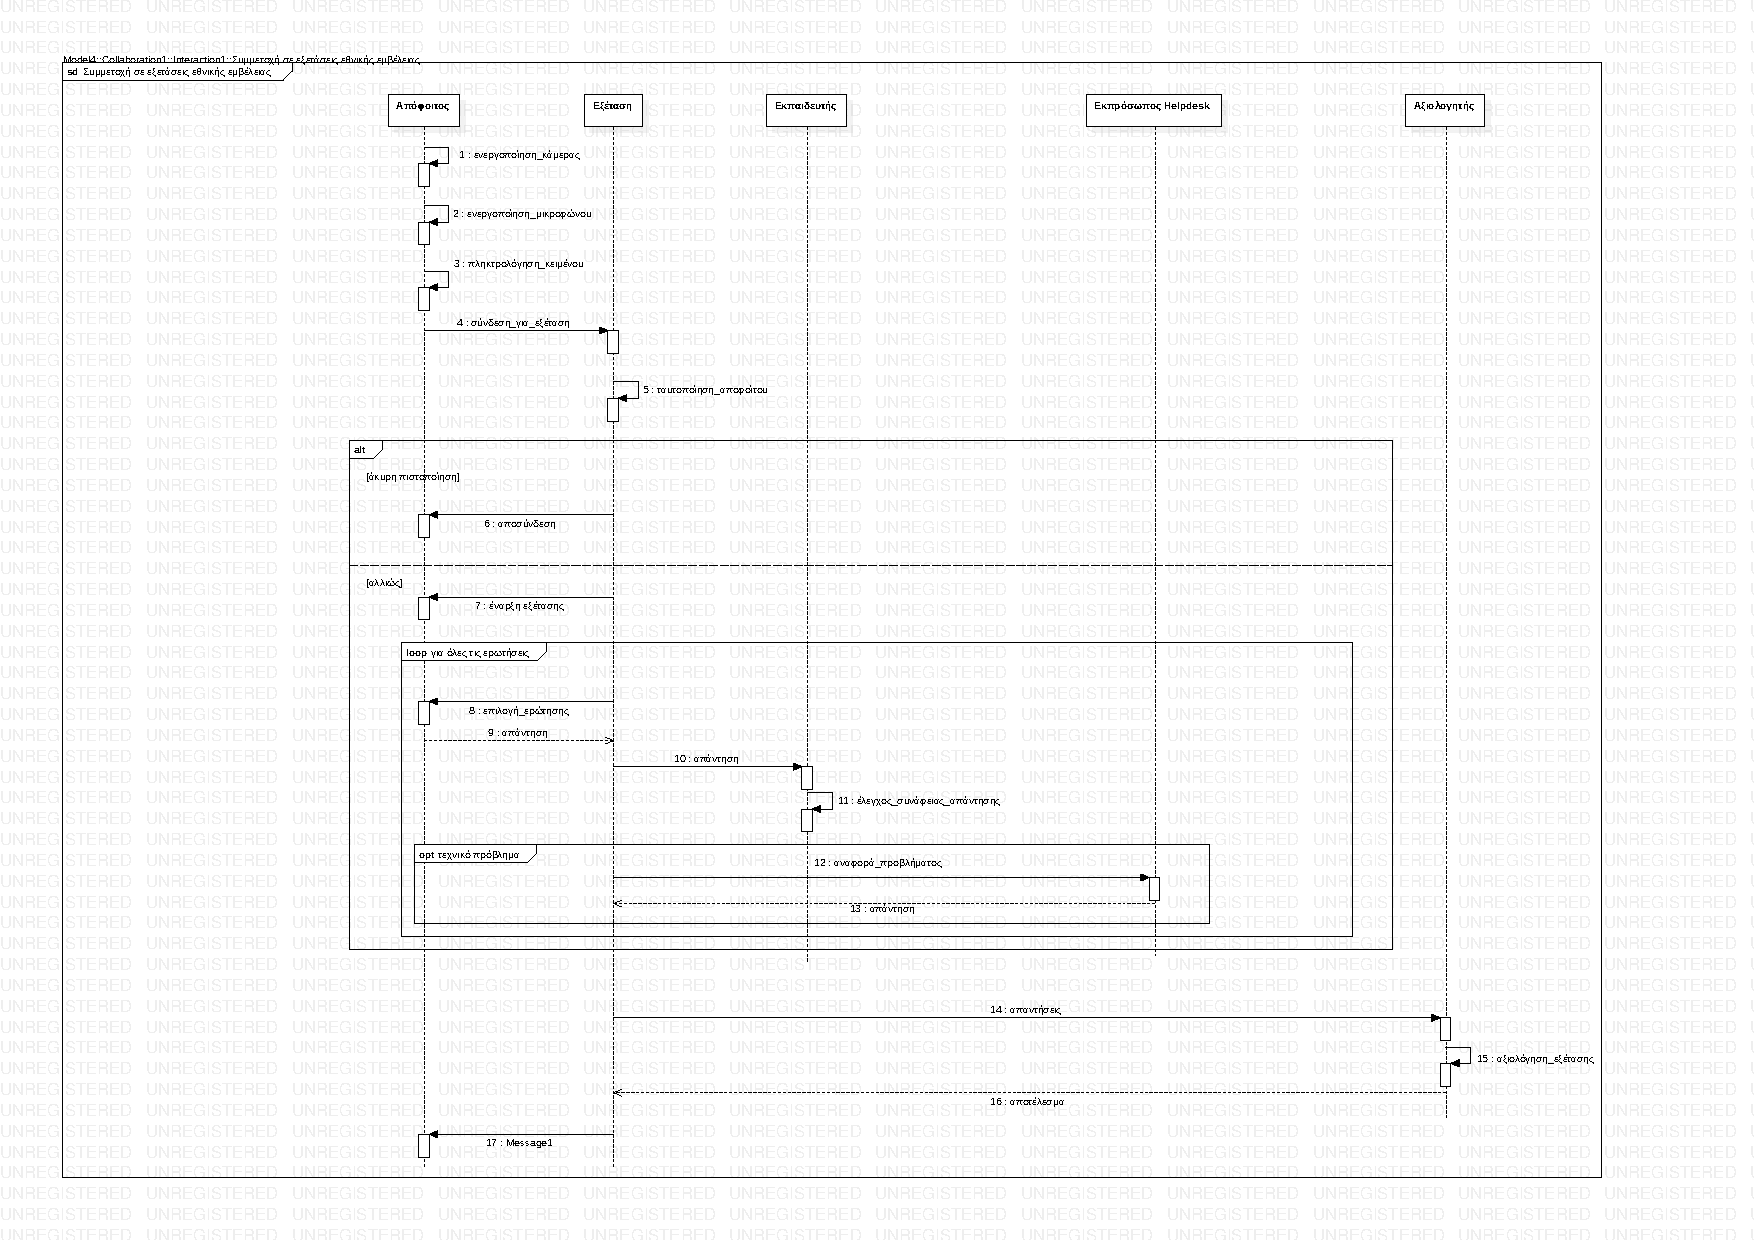
\includegraphics[width=.9\linewidth]{seq_4.pdf}
\end{center}
\end{itemize}

\subsection{Ερώτημα 5}
\label{sec:org5800110}

\subsubsection*{Διάγραμμα δραστηριοτήτων διαδικασίας 3}
\label{sec:org6c88e5f}
\begin{center}
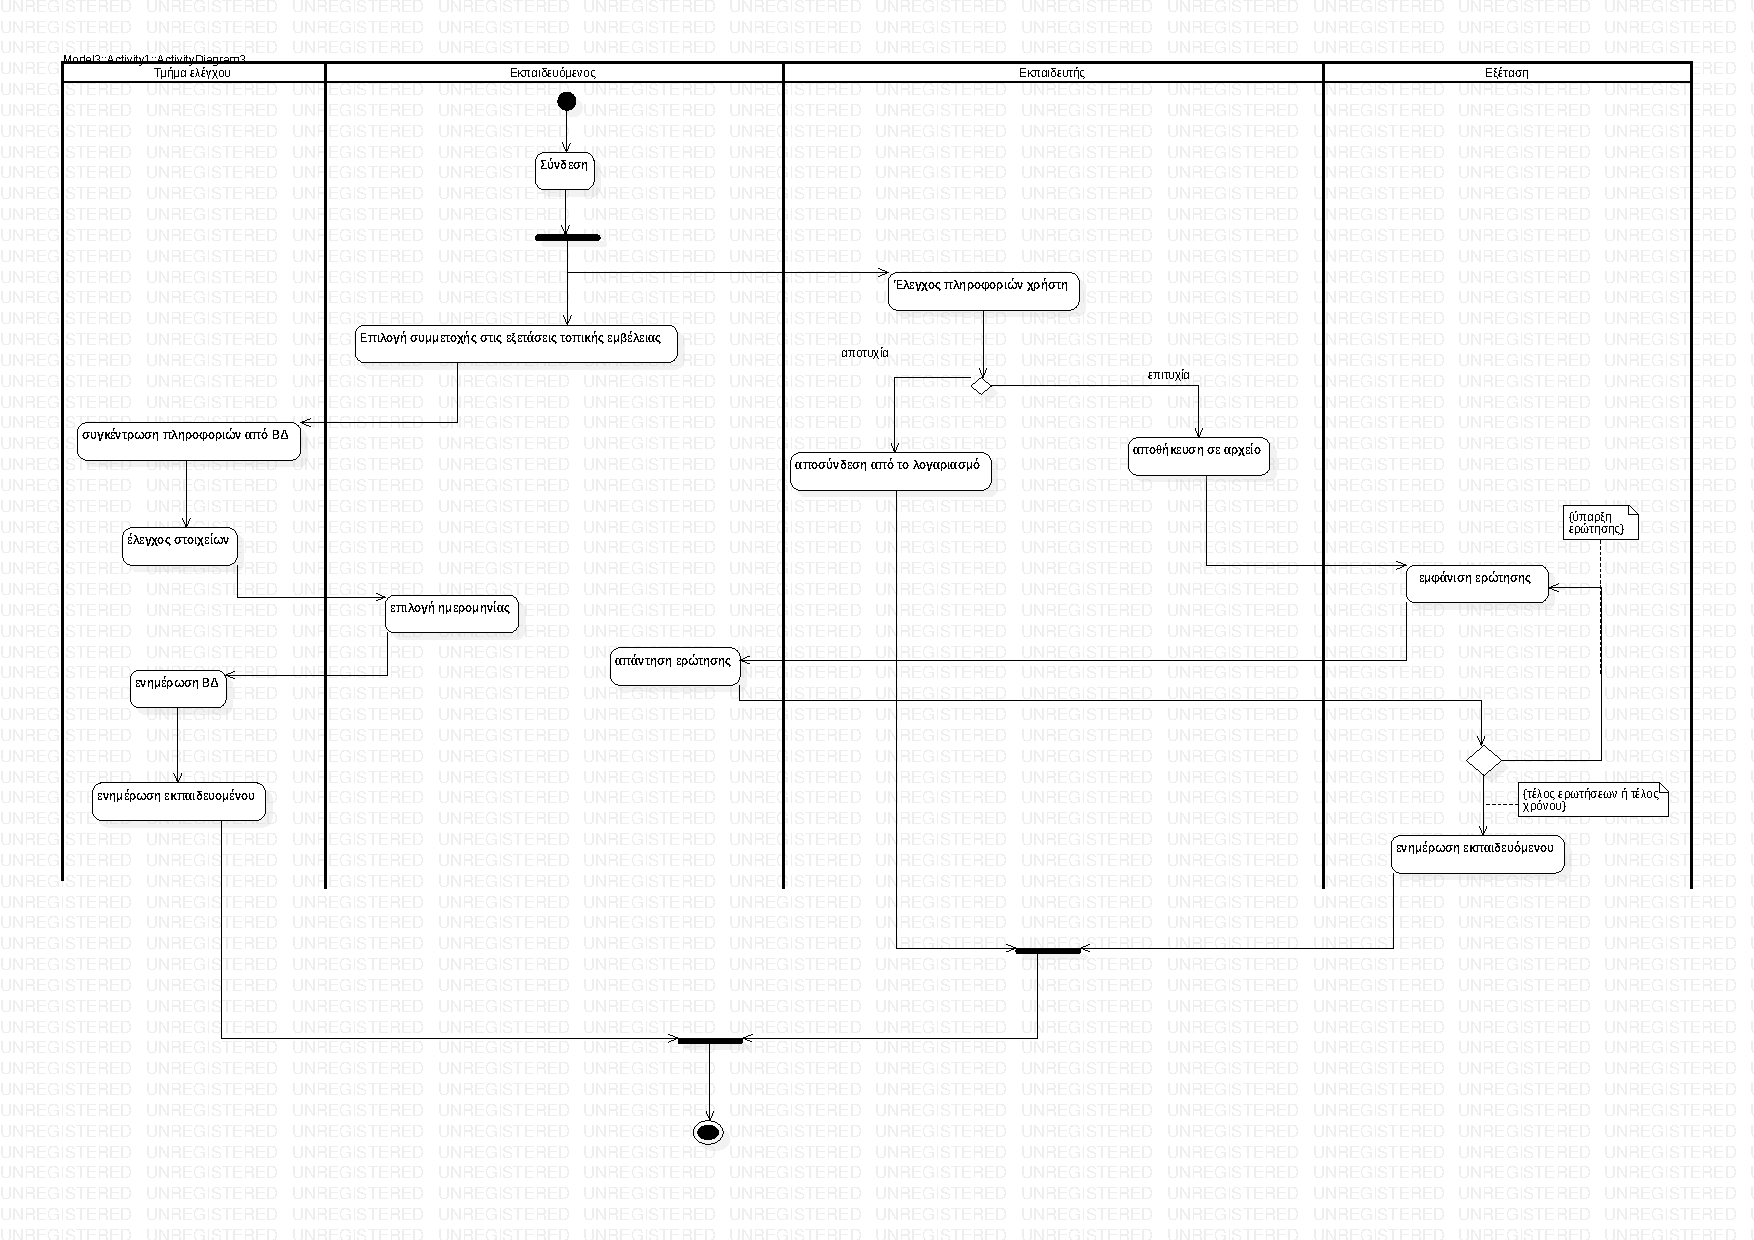
\includegraphics[width=.9\linewidth]{activity3.pdf}
\end{center}

\section{Μέρος Β: Δομημένη Ανάλυση}
\label{sec:org054ff8c}

\subsection{Ερώτημα 6}
\label{sec:orgfbab90d}

\subsubsection*{Επίπεδο αφαίρεσης 0 φορέα}
\label{sec:org92e79f1}
\begin{center}
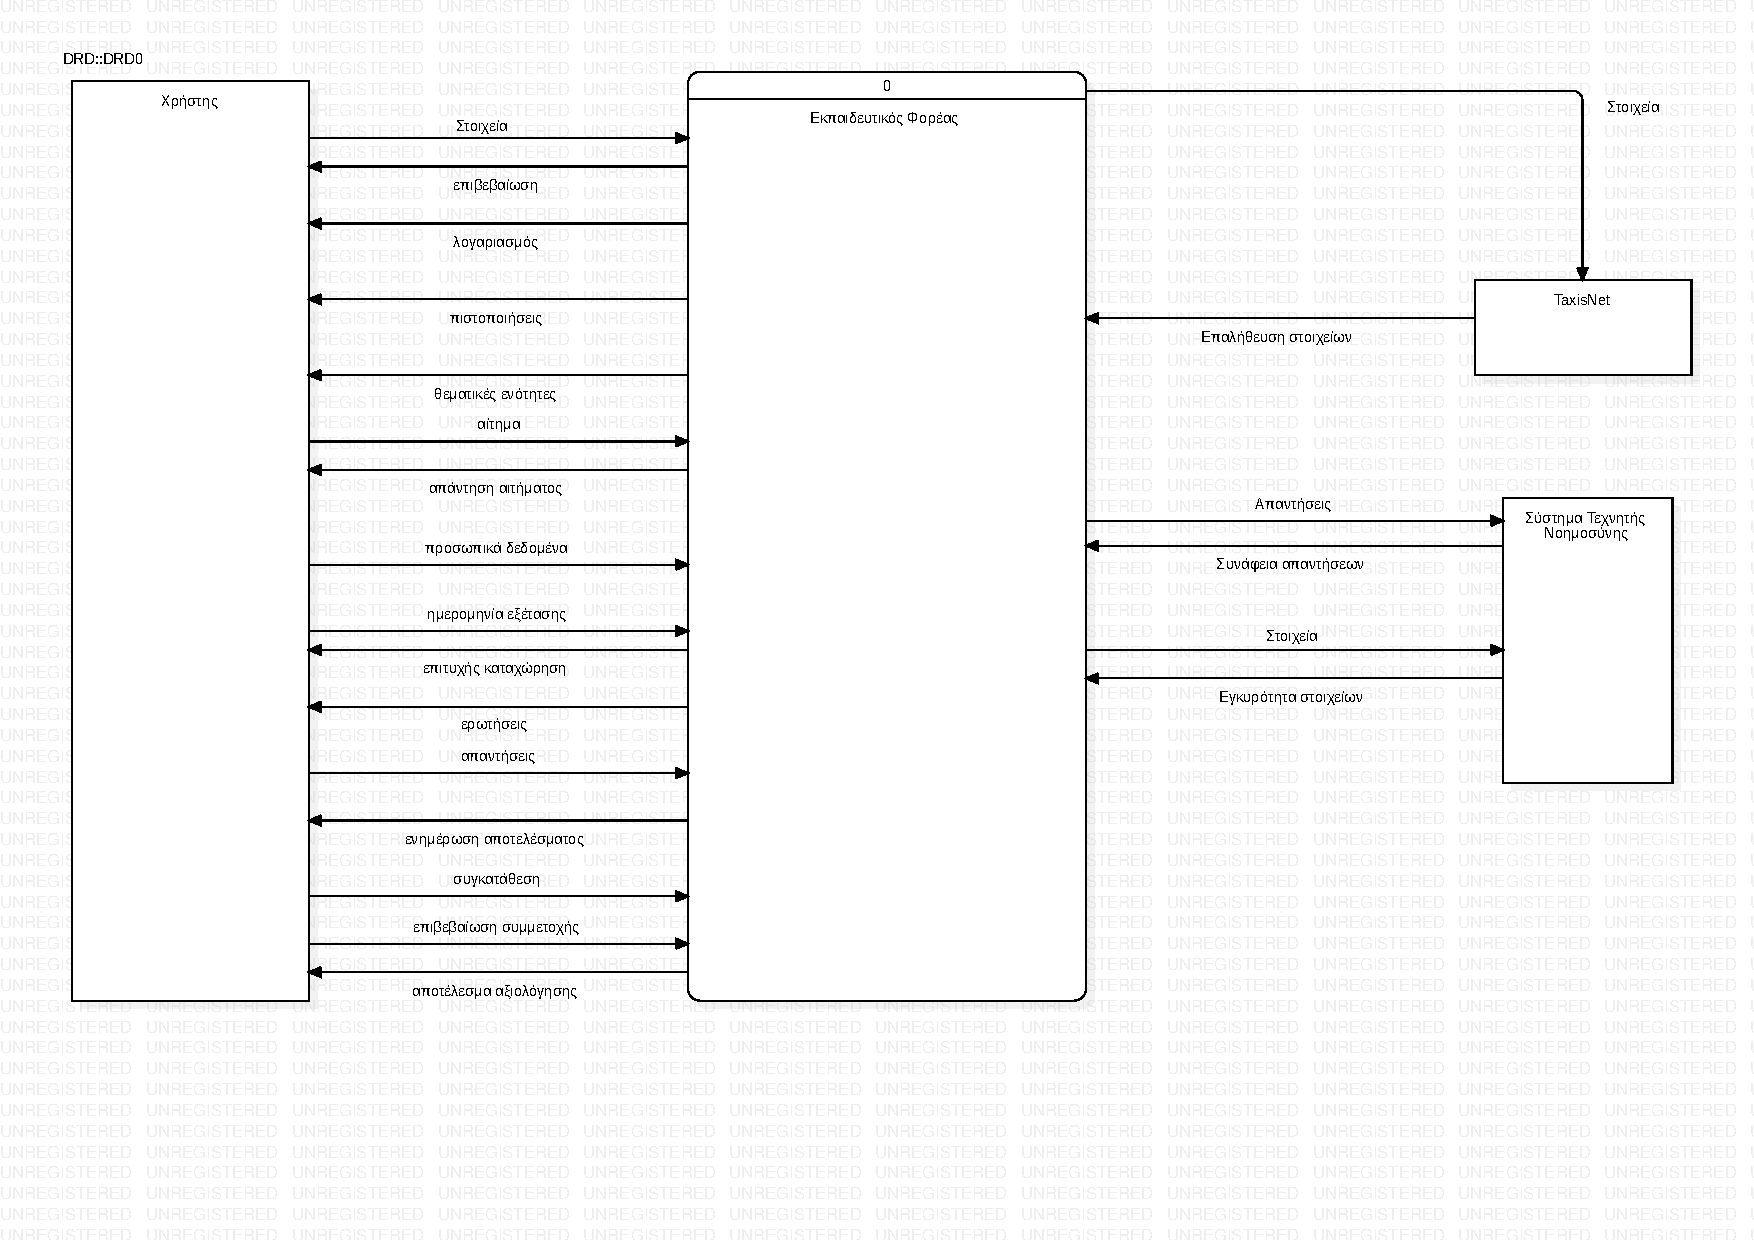
\includegraphics[width=.9\linewidth]{drd0.pdf}
\end{center}
\subsubsection*{Επίπεδο αφαίρεσης 1 φορέα}
\label{sec:orgbeeab31}
\begin{center}
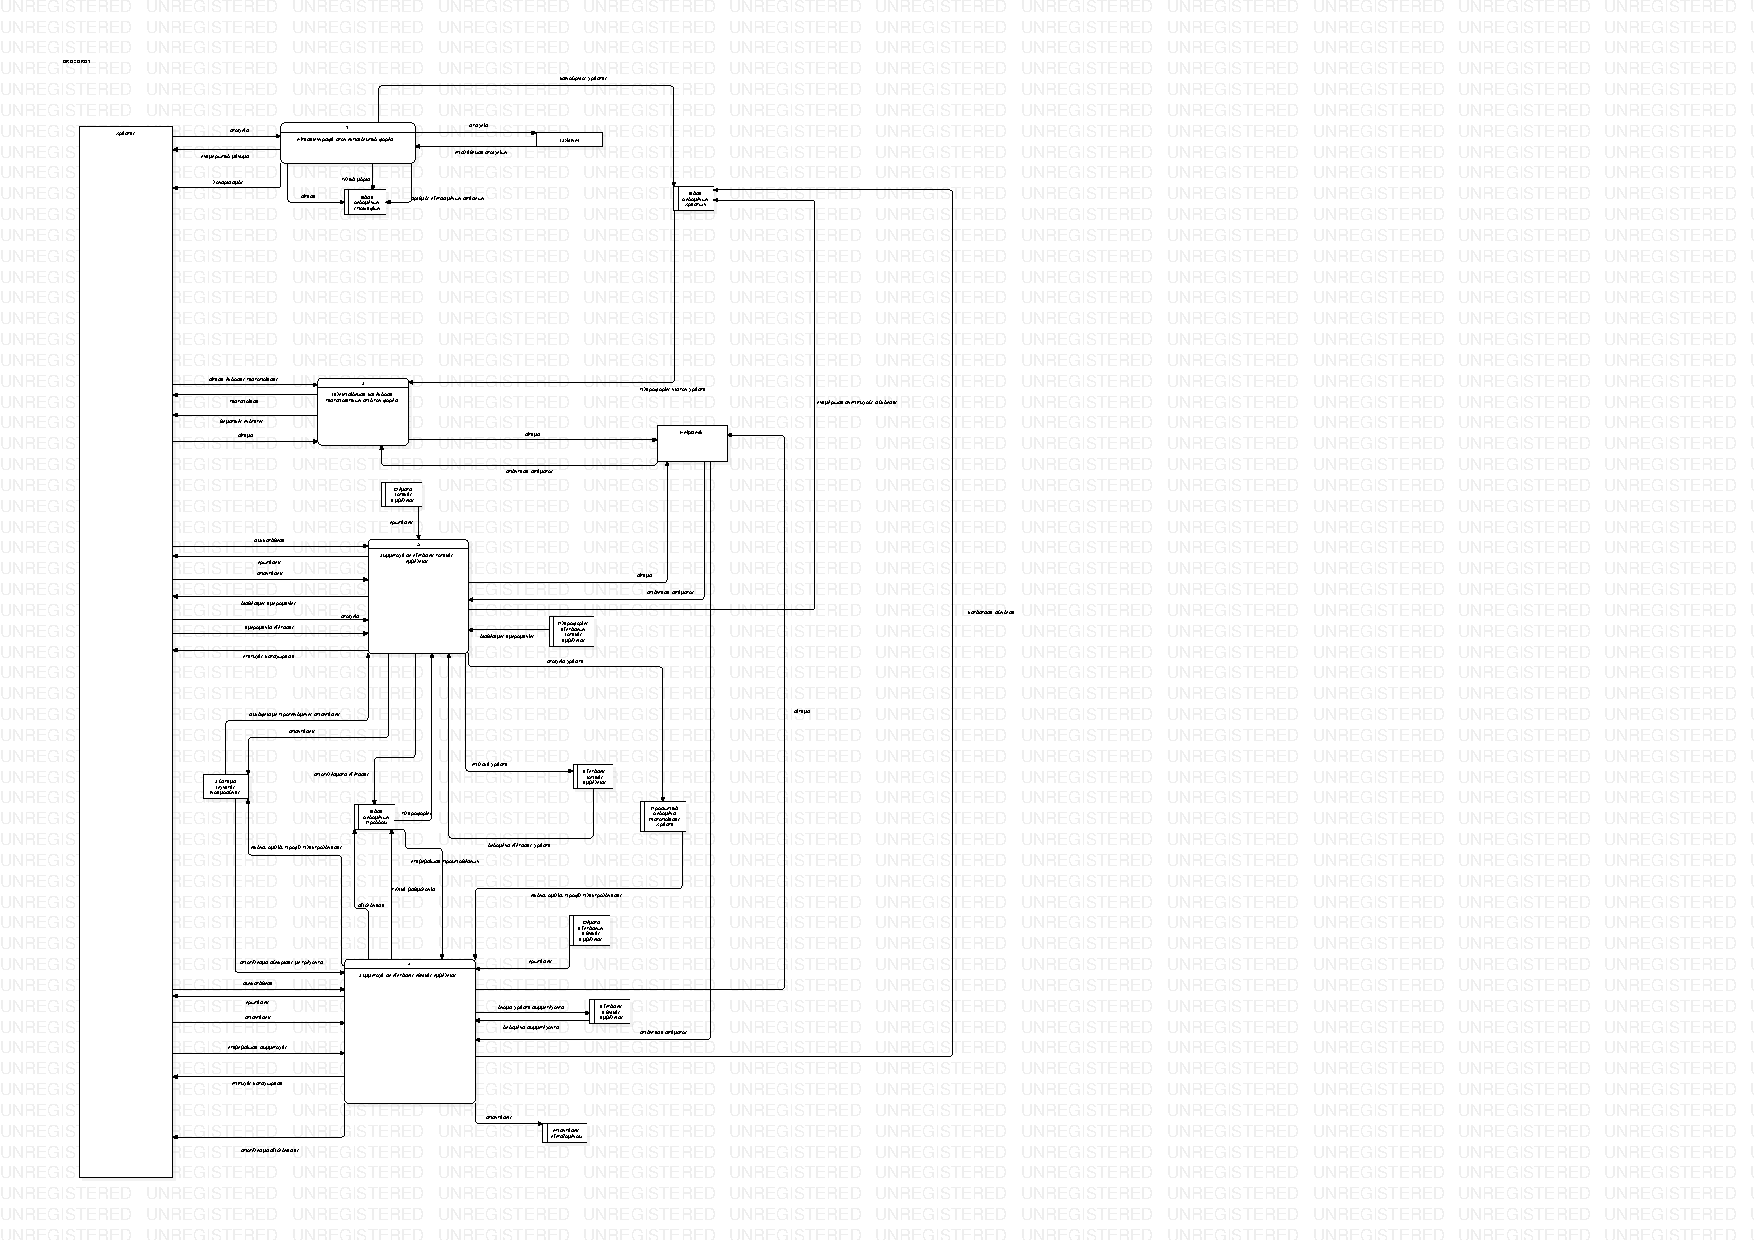
\includegraphics[width=.9\linewidth]{drd1.pdf}
\end{center}
\subsubsection*{Επίπεδο αφαίρεσης 2 διαδικασίας 2}
\label{sec:org8df7b21}
\begin{center}
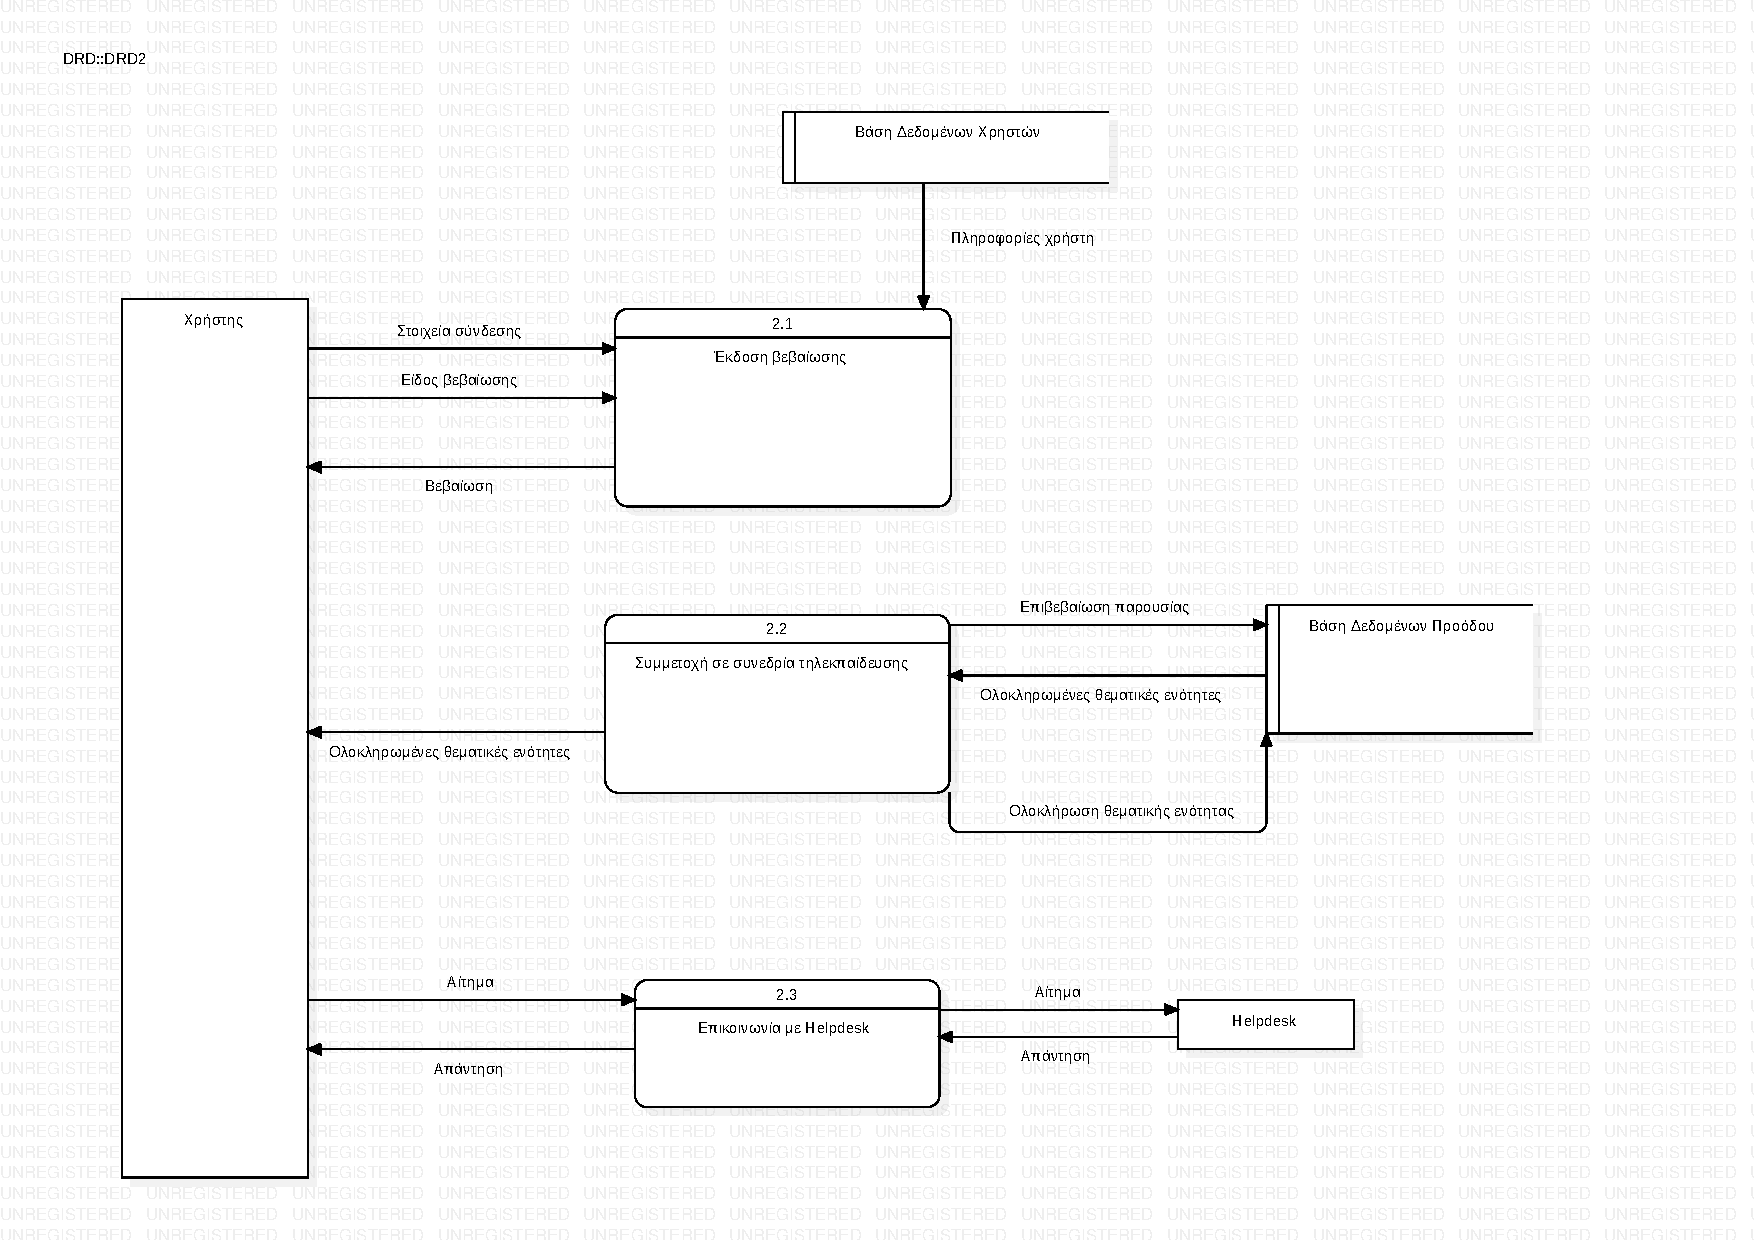
\includegraphics[width=.9\linewidth]{drd2.pdf}
\end{center}

\section{Επίλογος}
\label{sec:orgd061354}

Οι τελικές μας εντυπώσεις είναι πως η εργασία, αν και αρκετά βατή, θα μπορούσε να ανακοινωθεί νωρίτερα στο εξάμηνο. Ακόμα κι αν δεν είχε καλυφθεί νωρίτερα η ύλη, θα μπορούσαμε π.χ. να ασχοληθούμε με τα use case διαγράμματα νωρίτερα. Αυτό διότι η συγκεκριμένη περίοδος είναι περίοδος εργασιών για πολλά μαθήματα, η παραπάνω πρόταση θα διευκόλυνε την διαδικασία σε ένα βαθμό.

Επίσης, αν και όχι υπερβολικά δύσκολη, η εργασία ήταν μεγάλη σε όγκο και απαιτούσε πολλά διαγράμματα, κάτι που δεν συνάδει με το ποσοστό της στην τελική βαθμολογία.
\end{document}